\documentclass[12pt, eng, twoside, openany, final]{mgr}
% \documentclass[eng, printmode]{mgr}


% PREAMBULA


%% Language and font encodings
\usepackage[polish]{babel}
\usepackage[utf8x]{inputenc}
\usepackage[T1]{fontenc}

%% Sets page size and margins
\usepackage[a4paper,top=3cm,bottom=2cm,left=3cm,right=3cm,marginparwidth=1.75cm]{geometry}
%% \usepackage[a4paper, left=2.5cm, right=2.5cm, top=2.5cm, bottom=2.5cm, headsep=1.2cm]{geometry} -- Domski 

%% linki w spisie tresci, bibliografi
\usepackage[bookmarks=true,bookmarksnumbered=false,unicode=true,colorlinks=true,filecolor=black,linkcolor=black,urlcolor=black,citecolor=black]{hyperref}

\usepackage[colorinlistoftodos]{todonotes}


%OPEROWANIE NA OBRAZACH
\usepackage{graphicx}       % pakiet graficzny, umożliwiający m.in.
% import grafik w formacie eps
%\usepackage{epstopdf}		% pozwala na importowanie grafik w formacie eps
% przy użyciu pdflatex
\usepackage[update,prepend]{epstopdf}
\usepackage{rotating}       % pakiet umożliwiający obracanie rysunków
\usepackage{subfigure}      % pakiet umożliwiający tworzenie podrysunków
\usepackage{epic}           % pakiet umożliwiający rysowanie w środowisku latex
\usepackage{psfrag}         % pakiet umożliwiający podmianę łańcuchów znaków 
% w plikach eps
%\usepackage{curves}         % pakiet do wykreslania krzywych

%pakiety dodające dużo dodatkowych poleceń matematycznych
\usepackage{amsfonts}       % pakiet z rozmaitymi czcionkami matematycznymi
% \usepackage{amssymb}        % pakiet z rozmaitymi symbolami matematycznymi
\usepackage{amsmath}        % pakiet z rozmaitymi środowiskami matematycznymi

\usepackage{fp}             % pakiet z funkcjami operujacymi 
% na liczbach zmiennoprzecinkowych
\usepackage{calc}           % pakiet umożliwiający operacje arytmetyczne
% na tzw. licznikach (liczbach całkowitych)
\usepackage{leftidx}		% indeksy górne i dolne po lewej stronie

%definicje matematyczne
\providecommand{\abs}[1]{\lvert#1\rvert}
\providecommand{\norm}[1]{\lVert#1\rVert}

%pakiety wspomagające i poprawiające składanie tabel
\usepackage{supertabular}
\usepackage{array}
\usepackage{tabularx}
\usepackage{hhline}
\usepackage{longtable}		% wsparcie dla dlugich tabel
\usepackage{multicol}		% podzial strony na wiele kolumn

%pakiet do BibTex
\usepackage{cite}

\usepackage{url} %pakiet pozawalający na dodawanie adresów url w bibliografi

%pakiet wypisujący na marginesie etykiety równań i rysunków zdefiniowanych przez \label{}, chcąc wygenerować finalną wersję dokumentu wystarczy usunąć poniższą linię
%\usepackage{showlabels}

\usepackage{float}			% lepsza obsluga mechanizmow obiektow plywajacych
% wymuszenie wstawienia np. tabeli, obrazka w danym miejscu przez [H]

\usepackage{listings}       % pakiet dedykowany zrodlom programow
\usepackage{color}


\definecolor{dkgreen}{rgb}{0,0.6,0}
\definecolor{gray}{rgb}{0.5,0.5,0.5}
\definecolor{mauve}{rgb}{0.58,0,0.82}

\lstset{ %
	language=C++,                % the language of the code
	basicstyle=\scriptsize,           % the size of the fonts that are used for the code
	numbers=left,                   % where to put the line-numbers
	numberstyle=\tiny\color{gray},  % the style that is used for the line-numbers
	stepnumber=1,                   % the step between two line-numbers. If it's 1, each line 
	% will be numbered
	numbersep=5pt,                  % how far the line-numbers are from the code
	backgroundcolor=\color{white},      % choose the background color. You must add \usepackage{color}
	showspaces=false,               % show spaces adding particular underscores
	showstringspaces=false,         % underline spaces within strings
	showtabs=false,                 % show tabs within strings adding particular underscores
	%frame=single,                   % adds a frame around the code
	rulecolor=\color{black},        % if not set, the frame-color may be changed on line-breaks within not-black text (e.g. comments (green here))
	tabsize=2,                      % sets default tabsize to 2 spaces
	captionpos=b,                   % sets the caption-position to bottom
	breaklines=true,                % sets automatic line breaking
	breakatwhitespace=false,        % sets if automatic breaks should only happen at whitespace
	%title=\lstname,                   % show the filename of files included with \lstinputlisting;
	% also try caption instead of title
	keywordstyle=\color{blue},          % keyword style
	commentstyle=\color{dkgreen},       % comment style
	stringstyle=\color{mauve},         % string literal style
	escapeinside={\%*}{*)},            % if you want to add LaTeX within your code
	morekeywords={*,...},              % if you want to add more keywords to the set
	deletekeywords={...}              % if you want to delete keywords from the given language
}

%polish signs in lst code
\lstset{literate=%
	{ą}{{\k{a}}}1
	{ć}{{\'c}}1
	{ę}{{\k{e}}}1
	{ł}{{\l}}1
	{ń}{{\'n}}1
	{ó}{{\'o}}1
	{ś}{{\'s}}1
	{ż}{{\.z}}1
	{ź}{{\'z}}1
	{Ą}{{\k{A}}}1
	{Ć}{{\'C}}1
	{Ę}{{\k{E}}}1
	{Ł}{{\L}}1
	{Ń}{{\'N}}1
	{Ó}{{\'O}}1
	{Ś}{{\'S}}1
	{Ż}{{\.Z}}1
	{Ź}{{\'Z}}1
}

\usepackage{verbatim}       % pakiet dedykowany rozmaitym wydrukom tekstowym
\usepackage{ifthen}         % pakiet umożliwiający tworzenie prostych programów
% (m.in. zawiera instrukcje powtórzeniowe 
% i warunkowe)
\usepackage{upquote}		%normal quotations marks ' and `


% deklaracje wymagane przez pakiet theorem automatycznie ladowany w przypadku
% klasy dokumentu article
%
\newtheorem{Dn}{Definicja}[section]     % deklaracja srodowiska definicja
\newtheorem{La}[Dn]{Lemat}                % deklaracja srodowiska lemat
\newtheorem{Tm}[Dn]{Twierdzenie}          % deklaracja srodowiska twierdzenie
\newtheorem{Rk}[Dn]{Spostrze{\.z}enie}  % deklaracja srodowiska spostrzezenie
\newtheorem{Am}[Dn]{Algorytm}           % deklaracja srodowiska algorytm
\newtheorem{As}[Dn]{Za{\l}o{\.z}enie}   % deklaracja srodowiska zalozenie
\newtheorem{Pn}[Dn]{Propozycja}           % deklaracja srodowiska propozycja
\newtheorem{Py}[Dn]{W{\l}asno{\'s}{\'c}}  % deklaracja srodowiska wlasnosc
\newtheorem{Cy}[Dn]{Wniosek}              % deklaracja srodowiska wniosek
\newtheorem{Ee}[Dn]{Przyk{\l}ad}        % deklaracja srodowiska przyklad
\newtheorem{Ex}{{\'C}wiczenie}          % deklaracja srodowiska cwiczenie

\newtheorem{theorem}{Twierdzenie}[section] %nowe otoczenie do składania twierdzeń
%definicje własnych poleceń
\newcommand{\R}{I\!\!R} %symbol liczb rzeczywistych, działa tylko w trybie matematycznym

%helps to specify width of a column in table
%\begin{tabular}{|C{1cm}|c|c|c|c|c|c|c|c|c|c|}
%first column will have widht of 1cm
\newcolumntype{L}[1]{>{\raggedright\let\newline\\\arraybackslash\hspace{0pt}}m{#1}}
\newcolumntype{C}[1]{>{\centering\let\newline\\\arraybackslash\hspace{0pt}}m{#1}}
\newcolumntype{R}[1]{>{\raggedleft\let\newline\\\arraybackslash\hspace{0pt}}m{#1}}

\sloppy			%zawija bardzo długie linie

% \pagenumbering{gobble}% Remove page numbers (and reset to 1)
\usepackage{fancyhdr}
% \include{bibliografia}


% re-definiowane polecenie w celu przechowywania nazwiska autora, jego brak powoduje ostrzezenie (Warning) podczas przetwarzania.
\author{Piotr Szczpański} 

% re-definiowane polecenie w celu przechowywania polskiego tytułu pracy magisterskiej, jego brak powoduje ostrzezenie (Warning) podczas przetwarzania.
\title{Moduł sterownika oświetlenia LED} 


% polecenie zdefiniowane w celu przechowywania angielskiego tytułu pracy magisterskiej, jego brak powoduje ostrzezenie (Warning) podczas przetwarzania.
\engtitle{LED lighting controller module} 


% polecenie zdefiniowane w celu przechowywania danych osobowych prowadzacego prace, jego brak powoduje ostrzezenie (Warning) podczas przetwarzania.
\supervisor{dr inż. Antoni Izworski, W-4/K-8} 

% polecenie zdefiniowane w celu przechowywania danych osobowych opiekuna pracy. W przypadku gdy jest to ta sama osoba co \supervisor, nie nalezy uzywac tego polecenia. Jego brak usunie ze strony tytułowej zbedna informacje.
% \guardian{tytuł, Imie Nazwisko, jednostka} 


% polecenie zdefiniowane w celu przechowywania nazwy kierunku studiów, jego brak powoduje ostrzezenie (Warning) podczas przetwarzania.
\field{Automatyka i Robotyka (AIR)} 


% polecenie zdefiniowane w celu przechowywania nazwy specjalnosci studiów, jego brak powoduje ostrzezenie (Warning) podczas przetwarzania.
\specialisation{Robotyka (ARR)} 

% re-definiowane polecenie w celu przechowywania roku. Standardowo u dołu strony tytułowej wstawiany jest biezacy rok, uzycie tego polecenia pozwala wstawic dowolny rok.
\date{2018}
\usepackage{fancyhdr}

\begin{document}
\maketitle
\tableofcontents

\newpage

\pagestyle{fancy}
\fancyhead{} 
\fancyfoot{} 
\lhead{Politechnika Wrocławska Wydział Elektroniki}
\rfoot{\thepage}
\lfoot{Szczepański P., Moduł sterownika oświetlenia LED}


\chapter{Wstęp}
\thispagestyle{fancy}
    \section{Wprowadzenie}
    W dzisiejszych czasach oświetlenie w naszych domach oprócz funkcji czysto praktycznej, ma również służyć jako dekoracja i tworzyć integralną część wystroju. Oświetlenie LED stanowi znaczącą część rynku elektroniki konsumenckiej i w ciągu kilkunastu lat wyparła prawie całkowicie z użytku codziennego wolframowe żarówki i~lampy wyładowcze (potocznie zwane świetlówkami). Popularność technologii LED jest spowodowana głównie atrakcyjnymi cenami produktów i~znacząco większą sprawnością elektryczną oraz co za tym idzie niższym zużyciem energii elektrycznej.
    
    \section{Cel i zakres pracy}
    Celem pracy jest stworzenie nowoczesnego sterownika oświetlenia LED opartego na platformie mikrokontrolerowej. W szczególności cel pracy obejmuje: 
    \begin{itemize}
        \item stworzenie opisu i objaśnienia wykorzystanych technologii,
        \item opracowanie instrukcji obsługi modułu oraz dokumentacji dla użytkownika końcowego,
        \item opracowanie dokumentacji technicznej modułu,
        \item zaprojektowanie elektroniki, 
        \item zbudowanie modułu sterownika oświetlenia,
        \item wytworzenie oprogramowania oraz jego opisu funkcjonalnego.
    \end{itemize}
    Zakres pracy obejmuje stworzenie fizycznego modułu wraz z jego kompletną dokumentacją. W szczególności zakresem pracy jest:
    \begin{itemize}
        \item W zakresie opisu i objaśnienia wykorzystanych technologi jest podstawowe wprowadzenie w wykorzystane technologie.
        \item Zakresem opracowania instrukcji modułu jest stworzenie opisu dostępnych funkcjonalności oraz objaśnienie sposobu obsługi modułu.
        \item W zakresie dokumentacji technicznej jest opis stworzonego modułu, czyli opis poszczególnych elementów elektroniki.
        \item W zakresie zaprojektowania elektroniki jest dobór elementów pozwalających zrealizować postawione zadanie, stworzenie schematu elektrycznego oraz zaprojektowanie płytki drukowanej. Ponadto w opisie elektroniki powinna znaleźć się instrukcja montażu. 
        \item Zakres zbudowania modułu zawiera fizyczną konstrukcję na podstawie stworzonej wcześniej dokumentacji.
        \item W zakresie wytworzenia oprogramowania jest stworzenie oprogramowania odpowiedzialnego za graficzny interfejs użytkownika oraz oprogramowania odpowiedzialnego za obsługę sprzętu i logikę modułu. Do tego zakresu należy również stworzenie dokumentacji oprogramowania modułu.
    \end{itemize}
%
\chapter{Założenia projektowe}
\thispagestyle{fancy}  

    Tworzony moduł będzie oferował użytkownikowi możliwość sterowania kolorami i~jasnością trójkolorowego paska ledowego oraz sterowanie dwoma wyjściami przekaźnikowymi. Użytkownik będzie komunikował się z modułem przez czterocalowy dotykowy wyświetlacz. Interfejs będzie udostępniał możliwość ręcznej zmiany stanów podłączonego oświetlenia, zapisywania ustawień i czasowego wywoływania zapisanych scen oświetleniowych.\\*
    Gotowy moduł sterownika oświetlenia LED musi spełniać kryteria jakościowe, w~szczególności:
    \begin{itemize}
        \item częstotliwość odświeżania generowanego sygnału PWM sterującego pasek ledowy musi być na tyle wysoka, aby nie można było zaobserwować migotania,
        
        \item graficzny interfejs użytkownika powinien być przejrzysty, intuicyjny w obsłudze oraz na tyle responsywny, żeby
        obsługa modułu była komfortowa,
        
        \item moduł musi działać w ciągłości, tzn. konfiguracja wbudowanego systemu operacyjnego musi zabezpieczać sytuacje
        krytycznych błędów czasu działania, między innymi takich jak: desynchronizacja systemowego zegara, wyłączenie aplikacji interfejsu graficznego.
    \end{itemize}
%
\chapter{Opis wykorzystanych technologii}
\thispagestyle{fancy}
    \section{Raspberry Pi}
    Raspberry Pi jest serią jednopłytkowych komputerów opartych na rdzeniach ARM. Pod nazwą Raspberry Pi kryje się również olbrzymia społeczność rozwijająca oprogramowanie, tworząca biblioteki i materiały edukacyjne.
    W projekcie wykorzystano model \emph{Raspberry Pi Zero W V1.3} oparty na procesorze  \emph{Broadcom BCM2835 ARM11}\cite{RpiData}. Moduł wyposażony jest m.in. w 512MB pamięci RAM, moduł WiFi, moduł Bluetooth, port miniHDMI. Z uwagi na  duże możliwości techniczne oraz niską cenę, modułu ten jest powszechnie wykorzystywany przy prototypowaniu urządzeń elektronicznych IoT. 
    Na urządzeniu instalowany i uruchamiany jest system operacyjny. Producent dostarcza dedykowaną wersję Liunx'a Debian nazwaną Raspbian. Zawiera ona potrzebne biblioteki, jak i sterowniki do obsługi peryferiów mikroprocesora. Stosowanie systemu operacyjne Linux w zastosowaniach systemów wbudowanych pozwala tworzyć bardziej skomplikowane oprogramowanie, ułatwia tworzenie graficznych interfejsów użytkownika i pozwala na zdalne łączenie się z urządzeniem, pod warunkiem, że urządzenie wspiera to sprzętowo. Główną wadą korzystania z~systemu operacyjnego jest obsługa sprzętu mikroprocesora w czasie rzeczywistym, z~uwagi na procesy zachodzące w systemie np: przłączanie kontekstu wątków. 
    \section{Język C++}
    Język C++ powstawł w roku 1979 stworzony przez Bjarne Stroustrup'a jako rozszerzenie języka C, od tego czasu C++ doczekał się kilku standardów i od 2011 roku co 3 lata wydawana jest jego nowa wersja. C++ osiągną olbrzymią popularność dzięki swojej uniwersalności. W komercyjnych zastosowaniach przy tworzeniu oprogramowania na wbudowane systemy  często wypiera używanie czystego języka~C. C++ pozwala na tworzenie kodu zarówno nisko jak i wysokopoziomowego. Kod może być zarówno zorientowany obiektowo jak również czysto proceduralnie. W porównaniu do C, C++ pozwala w łatwiejszy sposób tworzyć reużywalny kod \cite{EffectiveModern}, dzięki mechanizmowi noszącemu nazwę polimorfizm. Biblioteka standardowa dostarcza bardzo dużo gotowych algorytmów, kontenerów itd. pozwalając skupić się na szybszym tworzeniu kodu spełniającego wymagania funkcjonalne.

    \newpage
    \section{Biblioteka QT i QML}
    QT jest zestawem bibliotek, których głównym celem jest tworzenie interfejsów graficznych aplikacji komputerowych. Ponadto QT dostarcza wiele narzędzi programistycznych pomagających rozwijać oprogramowanie. Oprócz zastosowań komputerowych QT daje możliwości tworzenia aplikacji na urządzenia wbudowane oraz mobilne i jest powszechnie używane przez takie firmy jak: LG, Mercedes-Benz. Biblioteka QT oparta jest o asynchroniczny mechanizm sygnałów i slotów, jest podstawą całego  jej działania. Po za możliwościami tworzenia interfejsów graficznych biblioteka dostarcza własne moduły, które pozwalają na: obsługę procesów, wykonywanie operacji na plikach, komunikację sieciową. Ponad to QT zawiera odpowiedniki kontenerów znajdujących się w STL\cite{EffectiveModern} (ang. Standard Template Library) z C++. Cała biblioteka napisana jest w sposób niezależny od architektury urządzeń docelowych, pozwalając na łatwe przenoszenie projektów. W pakiecie QT znajduje się zintegrowane środowisko programistyczne QT Creator (rysunek \ref{fig:qtc}). 
        \begin{figure}[H]
        \begin{center}
            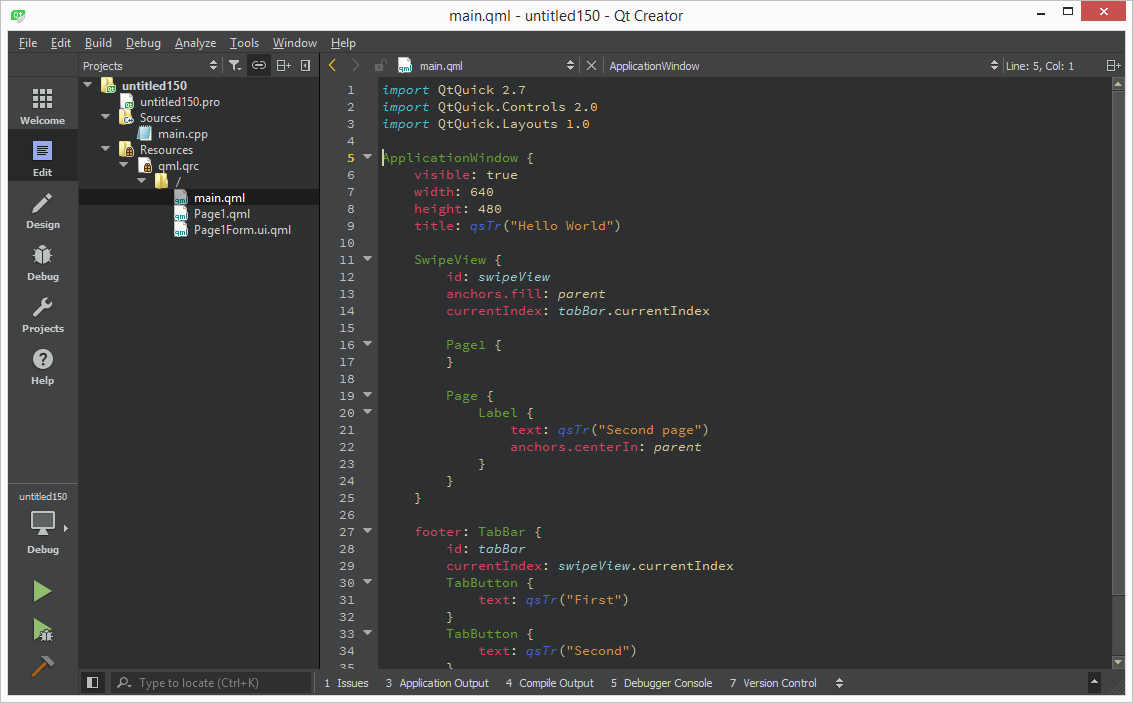
\includegraphics[width=0.8\textwidth]{qtc.png}
            \caption{Przykładowy widok w QT Creator }
            \label{fig:qtc}
        \end{center}
        \end{figure}
    \noindent Narzędzie to pozwala w łatwiejszy sposób tworzyć oprogramowanie korzystające z~biblioteki QT podpowiadając składnię poleceń i wyświetlając dokumentację. QT Creator umożliwia także na uruchamianie debbugera\cite{debugger}, wizualne tworzenie interfejsu użytkownika oraz kompilację skrośną\cite{RpiBeginner} (ang. cross-compile). Kompilacja skrośna polega na kompilowaniu i~tworzeniu pliku binarnego na stacji roboczej programisty i wgrywaniu samego pliku wykonywalnego na docelowe urządzenie wbudowane poprzez sieć Wi-Fi. Dzięki zastosowaniu takiego narzędzie czas wytwarzania oprogramowania znacznie się zmniejsza. 
     
%
\chapter{Dokumentacja użytkownika}
\thispagestyle{fancy}
    \section{Typowe wykorzystanie}
    \indent
    Przeznaczeniem modułu jest wykorzystanie w pomieszczeniu użytkowym, do sterowania intensywnością świecenia poszczególnych kolorów paska ledowego oraz do przełączania dwóch dwunastowoltowych wyjść przekaźnikowych. Wyjścia przekaźnikowe zostały umieszczone w projekcie tak aby pozwolić użytkownikowi podłączyć i~sterować np: stanem jednokolorowego paska LED, stanem żarówki LED lub zewnętrznym przekaźnikiem bądź stycznikiem.
    
    \section{Podłączanie zasilania i urządzeń wykonawczych}
    Moduł zasilany jest napięciem 12V i nie posiada zabezpieczenia przeciw odwrotnej polaryzacji zasilania. więc błędne podłączenie zasilacza może uszkodzić sterownik. 
    
        \begin{table}[H]
        \centering
        \begin{tabular}{ | m{18em} | m{1cm}| } 
        \hline
        Napięcie zasilania & 12V \\ 
        \hline
        Sumaryczny prąd wyjściowy & 15A \\ 
        \hline
        Maksymalny prąd wyjścia przekaźnikowego &10A\\
        \hline
        Maksymalny sumaryczny prąd pojedynczego wyjścia przekaźnikowego &14A\\
        \hline
        Prąd wyjścia sterownika paska led &12A\\
        \hline
        \end{tabular}
        \caption{Parametry elektryczne modułu}
        \label{tab:param}
        \end{table}
    \noindent
    Wartości zawarte w tabeli \ref{tab:param} gwarantują poprawne działanie modułu. 
    Należy pamiętać, że podłączone obciążenie nie może przekraczać maksymalnej mocy zasilacza.Ponadto maksymalny prąd zasilacz powinien wynosić przynajmniej \textbf{450mA}, więcej niż potrzebuje tego obciążenie, gdyż należy doliczyć zapotrzebowanie Raspberry Pi z wyświetlaczem. Podane \textbf{450mA} jest wartością bezpieczną i nie znaczy to, że moduł pobiera w trakcie swojego działania taki prąd.\newpage \noindent Zasilacz należy podłączyć do złącza \emph{J5}, wyjścia przekaźnikowe są oznaczone symbolami \emph{J3}, \emph{J4}, a sterownik paska ledowego \emph{J1J2}. Sposób podłączenie paska led jest oznaczony bezpośrednio na płytce, przykładem jest rysunek \ref{fig:strip}. 
        \begin{figure}[H]
        \begin{center}
            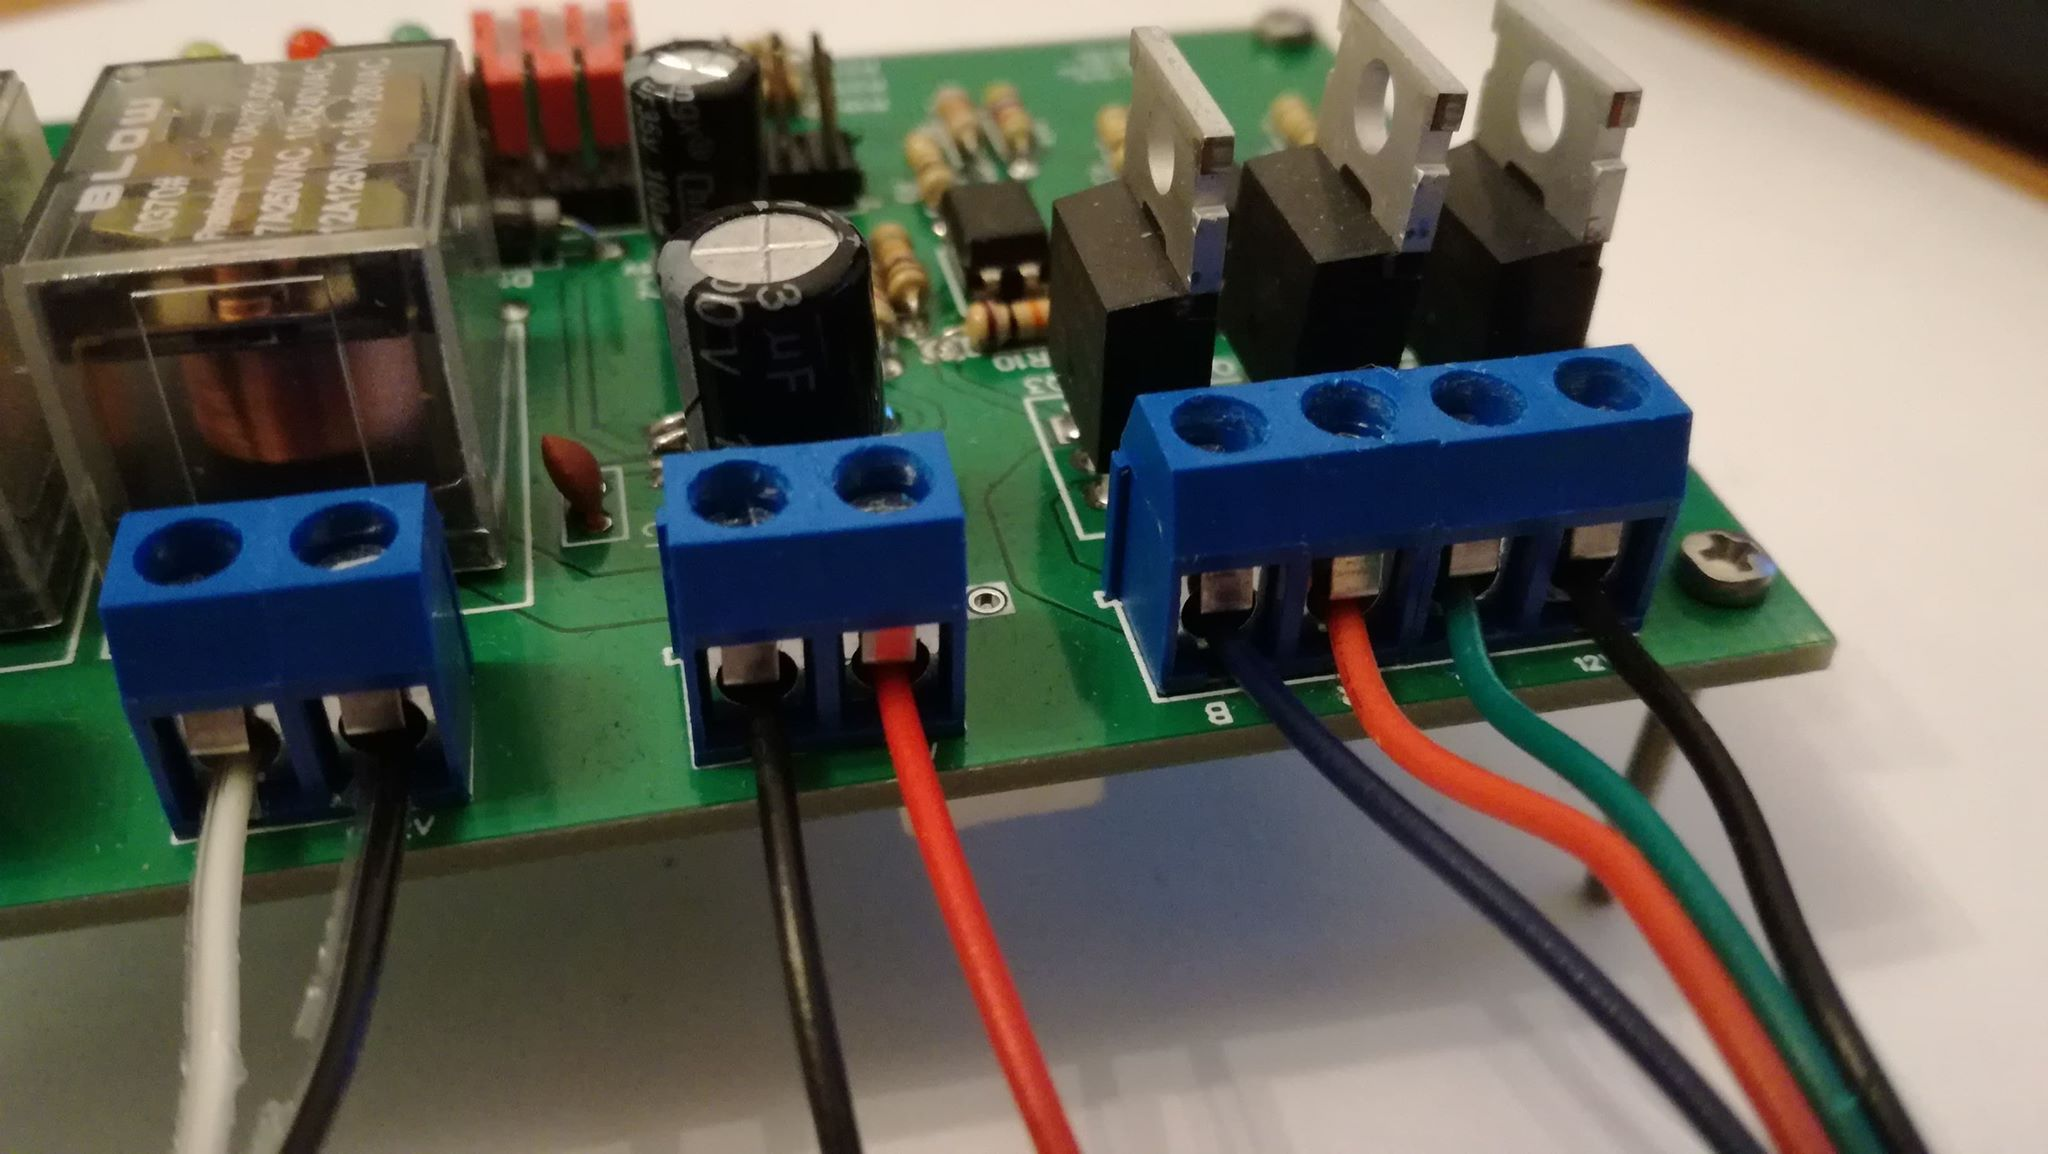
\includegraphics[width=0.65\textwidth]{podlaczone.jpg}
            \caption{Przykład podłączenia zasilania, paska led oraz żarówki led}
        \end{center}
        \end{figure}
        \begin{figure}[H]
        \begin{center}
            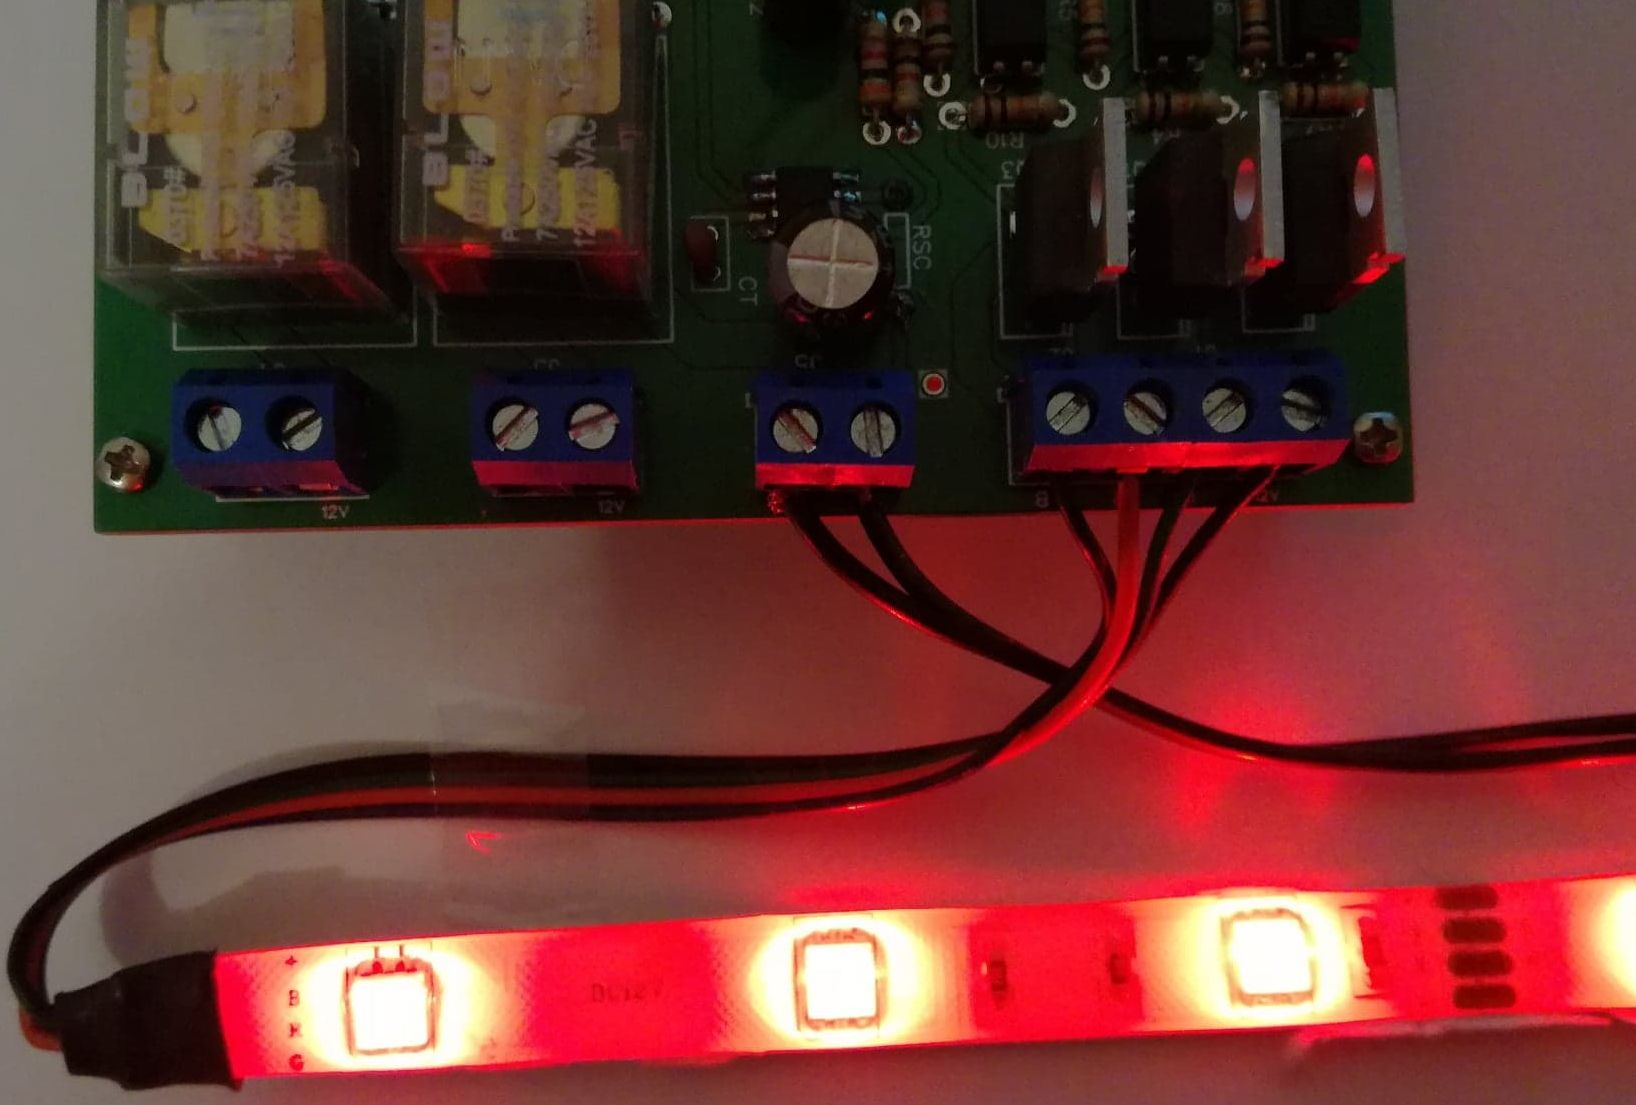
\includegraphics[width=0.65\textwidth]{zpaskiem.jpg}
            \caption{Przykład podłączenia i swiecenia paska led}
            \label{fig:strip}
        \end{center}
        \end{figure}
    \newpage
    
    \section{Opis interfejsu graficznego}
    Interfejs graficzny zbudowany jest jako seria widoków. Aby aktywować kolejny widok należy horyzontalnie przesunąć rysikiem po wyświetlaczu dotykowym, zgodnie z żądanym kierunkiem zmiany widoku. Takie rozwiązanie jest intuicyjne, gdyż dokładnie w takim sposób obsługuje się interfejsy graficzne w telefonach komórkowych (smartfonach), więc jest to zachowanie do którego przeciętny użytkownik jest przyzwyczajony.
    Widokiem startowym jest widok kontroli ręcznej wyjść modułu, przedstawiony na rysunku \ref{fig:screen}.
        \begin{figure}[H]
        \begin{center}
            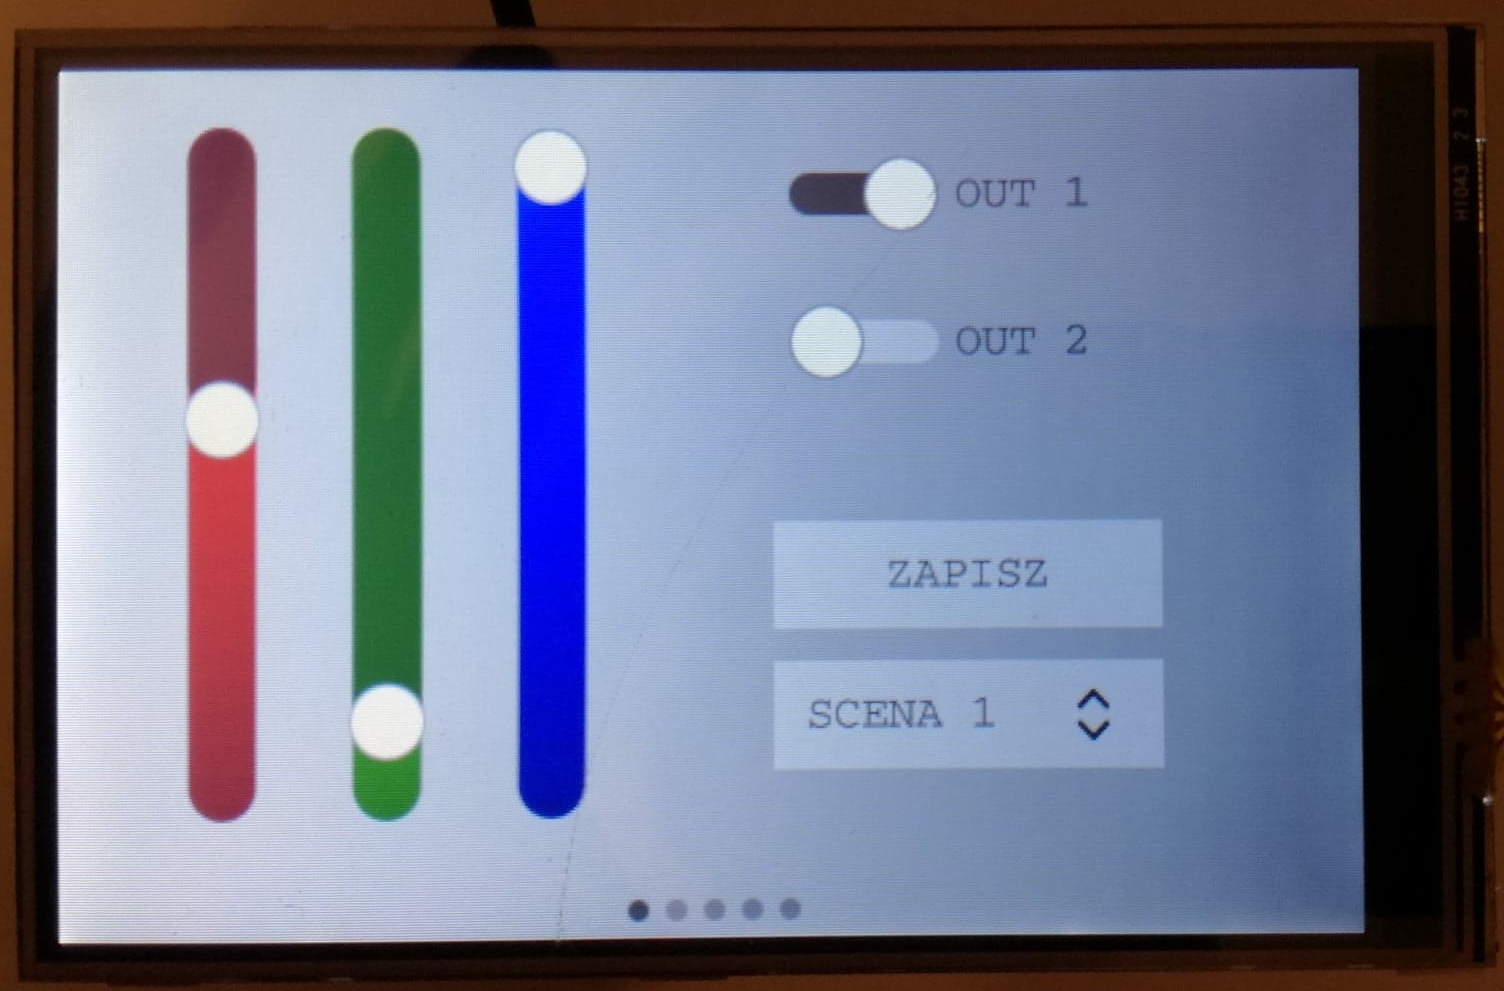
\includegraphics[width=0.5\textwidth]{ui_live.jpg}
            \caption{Zdjęcie ekranu z interfejsem graficznym}
            \label{fig:screen}
        \end{center}
        \end{figure}
    
\noindent    Położenie aktywnego widoku jest prezentowane w dolnej części interfejsu (rysunek \ref{fig:ind}). Ciemniejsza kropka oznacza aktywny region, pozostałe pokazują dostępne regiony.
        \begin{figure}[H]
        \begin{center}
            
\includegraphics[width=0.25\textwidth]{ui_pageind.jpg}
            \caption{Wskaźnik widoków}
            \label{fig:ind}
        \end{center}
        \end{figure}
    \newpage
    
    \section{Opis funkcji}
        Sterownik udostępnia 4 funkcje sterowania wyjściami. Pozwalają one na:+ ręczne sterowanie wyjściami wraz z możliwością zapisania konfiguracji w pamięci sterownika, przełączania między zapisanymi scenami, czasowe wywoływanie scen i animacji zapisanych w sterowniku oraz włączanie animacji paska led wraz z możliwością sterownia prędkością zmiany kolorów.
        \subsection{Tworzenie scen}
        Tworzenie scen odbywa się przez zapisanie aktualnych ustawień sterownika. Sterownik udostępnia możliwość zapisania  9 scen. Każda ze scen przechowuje dane o~ustawieniach wyjść paska ledowego oraz stanie wyjść przekaźnikowych. 

            \begin{figure}[H]
            \begin{center}
                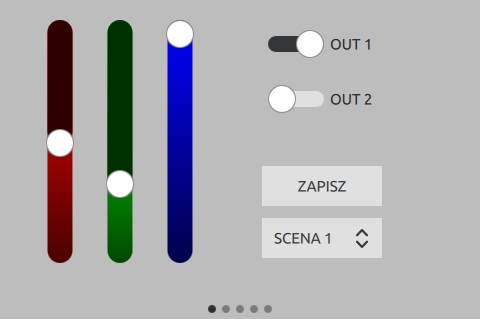
\includegraphics[width=0.45\textwidth]{ui_manualTab.jpg}
                \caption{Widok nr 1: Ekran użytkownika podczas tworzenia scen}
                \label{fig:view1}
            \end{center}
            \end{figure}
            \noindent Tworzenie scen należy rozpocząć od ręcznego ustawienia żądanych stanów wyjść, poprzez przesuwanie rysikiem po ekranie i~obserwację podłączonego paska ledowego. Aby zapisać obecne ustawienia w pamięci sterownika należy wybrać z pola Rys \ref{fig:box} numer sceny, pod którą mają one zostać zapamiętane. Jeśli w danej scenie występują zapisane ustawienia to zostaną one nadpisane.
            
            \begin{figure}[!h]
        	\centering
        	\begin{minipage}[t]{3cm}
        		\centering
        		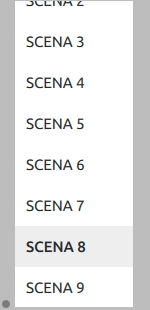
\includegraphics[scale=0.4]{ui_box.jpg}
        		\caption{Pole wyboru scen} \label{fig:box} 
        	\end{minipage}
        	\hspace{3cm}
        	\begin{minipage}[t]{5cm}
        		\centering
        		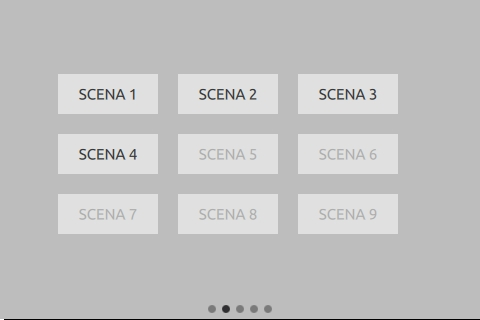
\includegraphics[scale=0.4]{ui_sceneTAB.jpg}
        		\caption{Widok nr 2: Ekran użytkownika podczas wyboru zapisanych scen} \label{fig:scene} 
        	\end{minipage}
        \end{figure}
            
        \noindent Widok nr 2 (rysunek \ref{fig:box}) pozwala użytkownikowi wybrać z zapisanych scen. Widok ten pojawia się na ekranie po naciśnięciu pola pod przyciskiem \emph{ZAPISZ} na rysunku \ref{fig:view1} Jak można zaobserwować na Rys \ref{fig:scene}, aktywne są wyłącznie przyciski, w których sceny zawierają dane. Przy pierwszym uruchomieniu modułu dostępne są cztery przykładowe sceny.
        
        \subsection{Tworzenie zdarzeń aktywowanych czasowych}
        Funkcja ta pozwala na stworzenie dwóch alarmów, które o zadanym czasie będą aktywowały wybraną funkcję. 
            \begin{figure}[H]
            \begin{center}
                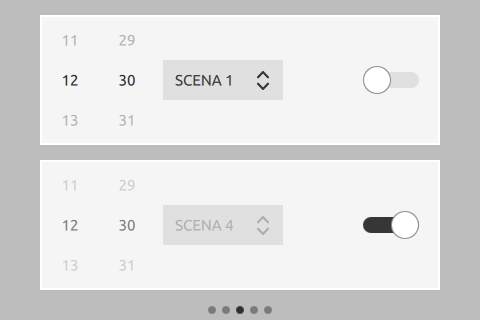
\includegraphics[width=0.5\textwidth]{ui_time.jpg}
                \caption{Widok nr 3: Ekran alarmów czasowych} 
                \label{fig:view3}
            \end{center}
            \end{figure}
            
        W lewej części widoku należy wybrać godzinę aktywacji, w środkowej części wybiera się funkcję, która ma zostać wywołana. Przełącznik po prawej stronie aktywuje alarm i w po jego aktywacji, tak jak widać na dolnym alarmie, kontrolki stają się nieedytowalne. Alarmy mają priorytet w wywołaniu nad innymi funkcjami, więc~należy pamiętać o ich ustawieniu.
        
        \subsection{Aktywacja animacji}
        Funkcja ta pozwoli włączyć animacje paska led, można wybrać z 10 gotowych, wcześniej zaprogramowanych. Obecna wersja oprogramowania nie pozwala użytkownikowi tworzyć własnych sekwencji kolorów. Użytkownik przy każdej sekwencji może wybrać szybkość jej wykonywanie w tym celu służy suwak znajdujący się na środku widoku, widoczne na rysunku \ref{fig:view5}.
            \begin{figure}[H]
            \begin{center}
                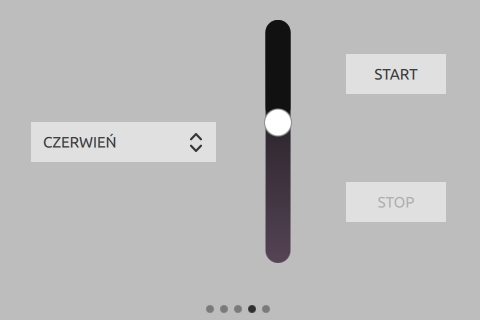
\includegraphics[width=0.5\textwidth]{ui_animation.jpg}
                \caption{Widok nr 4: Ekran ustawień animacji}
                \label{fig:view5}
            \end{center}
            \end{figure}
        
        \subsection{Sterowanie stanami}
        Na ostatniej pozycji w przesuwalnym menu (Rysunek \ref{fig:view6}), znajduje się widok służący włączaniu i wyłączaniu wyjść. Ma on najwyższy priorytet, więc w momencie aktywacji alarmu lub sterowania ręcznego, gdy wyjście będzie wyłączone w tym widoku inne operacje będą ignorowane. W przypadku przełącznika stanu dla paska ledowego, gdy wszystkie jego ustawienia będą równe zero a użytkownik użyje przełącznika to będzie on nadal wyłączony. Przełącznik ten służy do wyłączania wybranej sceny lub animacji. Nie powoduje on jednak zatrzymania animacji.
            \begin{figure}[H]
            \begin{center}
                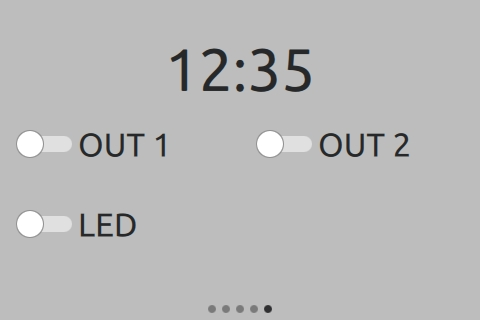
\includegraphics[width=0.5\textwidth]{ui_global.jpg}
                \caption{Widok nr 5: Ekran globalnych przełączników wyjść} \label{fig:view6}
            \end{center}
            \end{figure}
    
    
    \newpage

\chapter{Dokumentacja serwisowa}
\thispagestyle{fancy}
    \section{Budowa modułu}
    Sterownik składa się z zaprojektowanej płytki z elektroniką wykonawczą i stabilizatorem napięcia, połączonej wielożyłowym kablem z modułem \emph{Raspberry Pi}(rysunek \ref{fig:rpi1}), do którego, za pomocą listwy goldpin, podłączony jest wyświetlacz dotykowy, widoczne na rysunku \ref{fig:rpi_lcd}.
        \begin{figure}[H]
        \begin{center}
            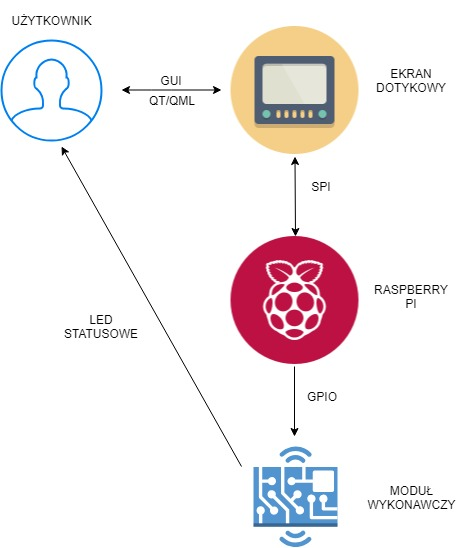
\includegraphics[width=0.45\textwidth]{diagram.jpg}
            \caption{Schemat ideowy modułu}
        \end{center}
        \end{figure}
        
       
        \begin{figure}[!h]
        	\centering
        	\begin{minipage}[t]{5cm}
        		\centering
        		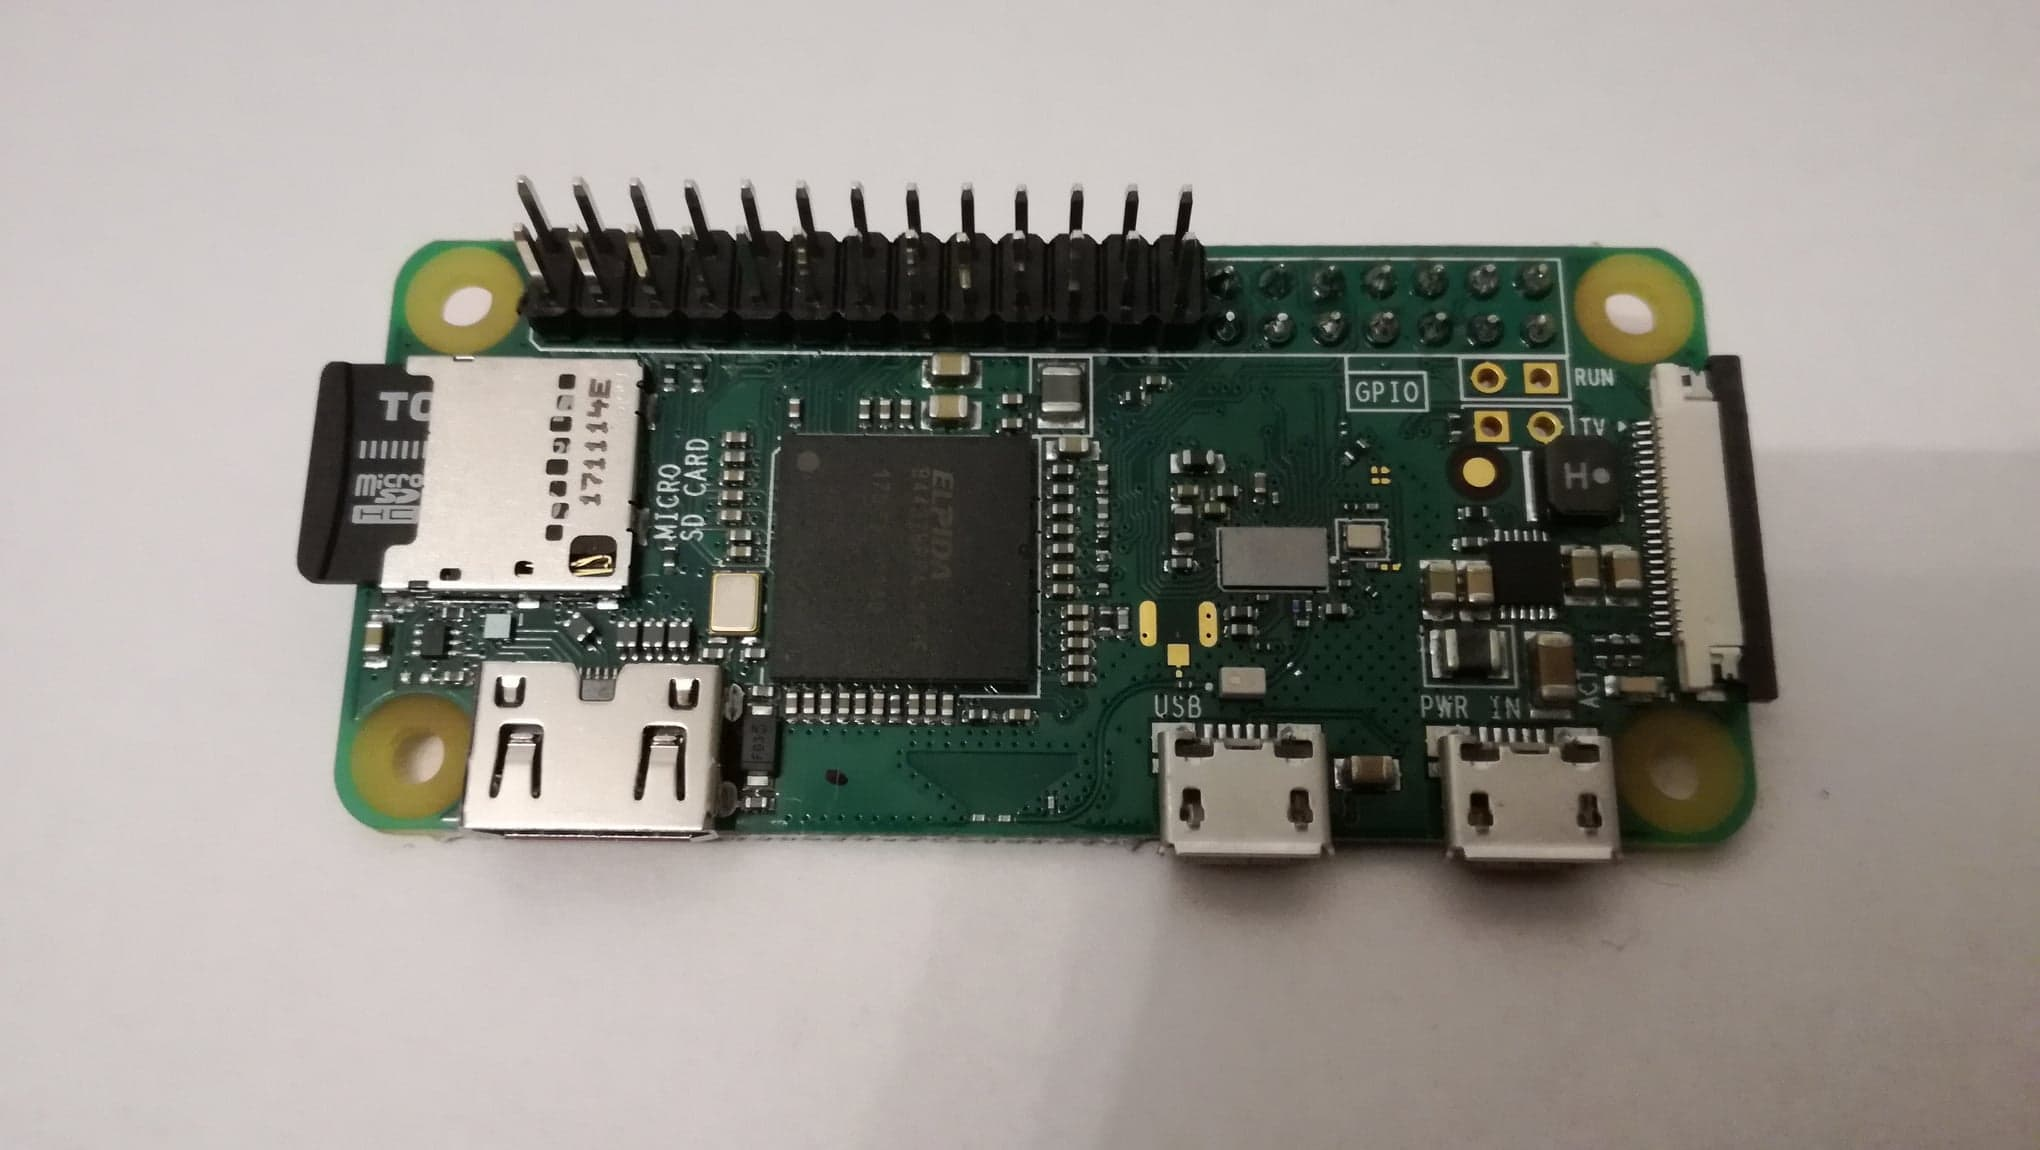
\includegraphics[scale=0.1]{rpi_goldpin.jpg}
        		\caption{Raspberry Pi z przylutowanymi złączami goldpin} \label{fig:rpi1} 
        	\end{minipage}
        	\hspace{3cm}
        	\begin{minipage}[t]{5cm}
        		\centering
        		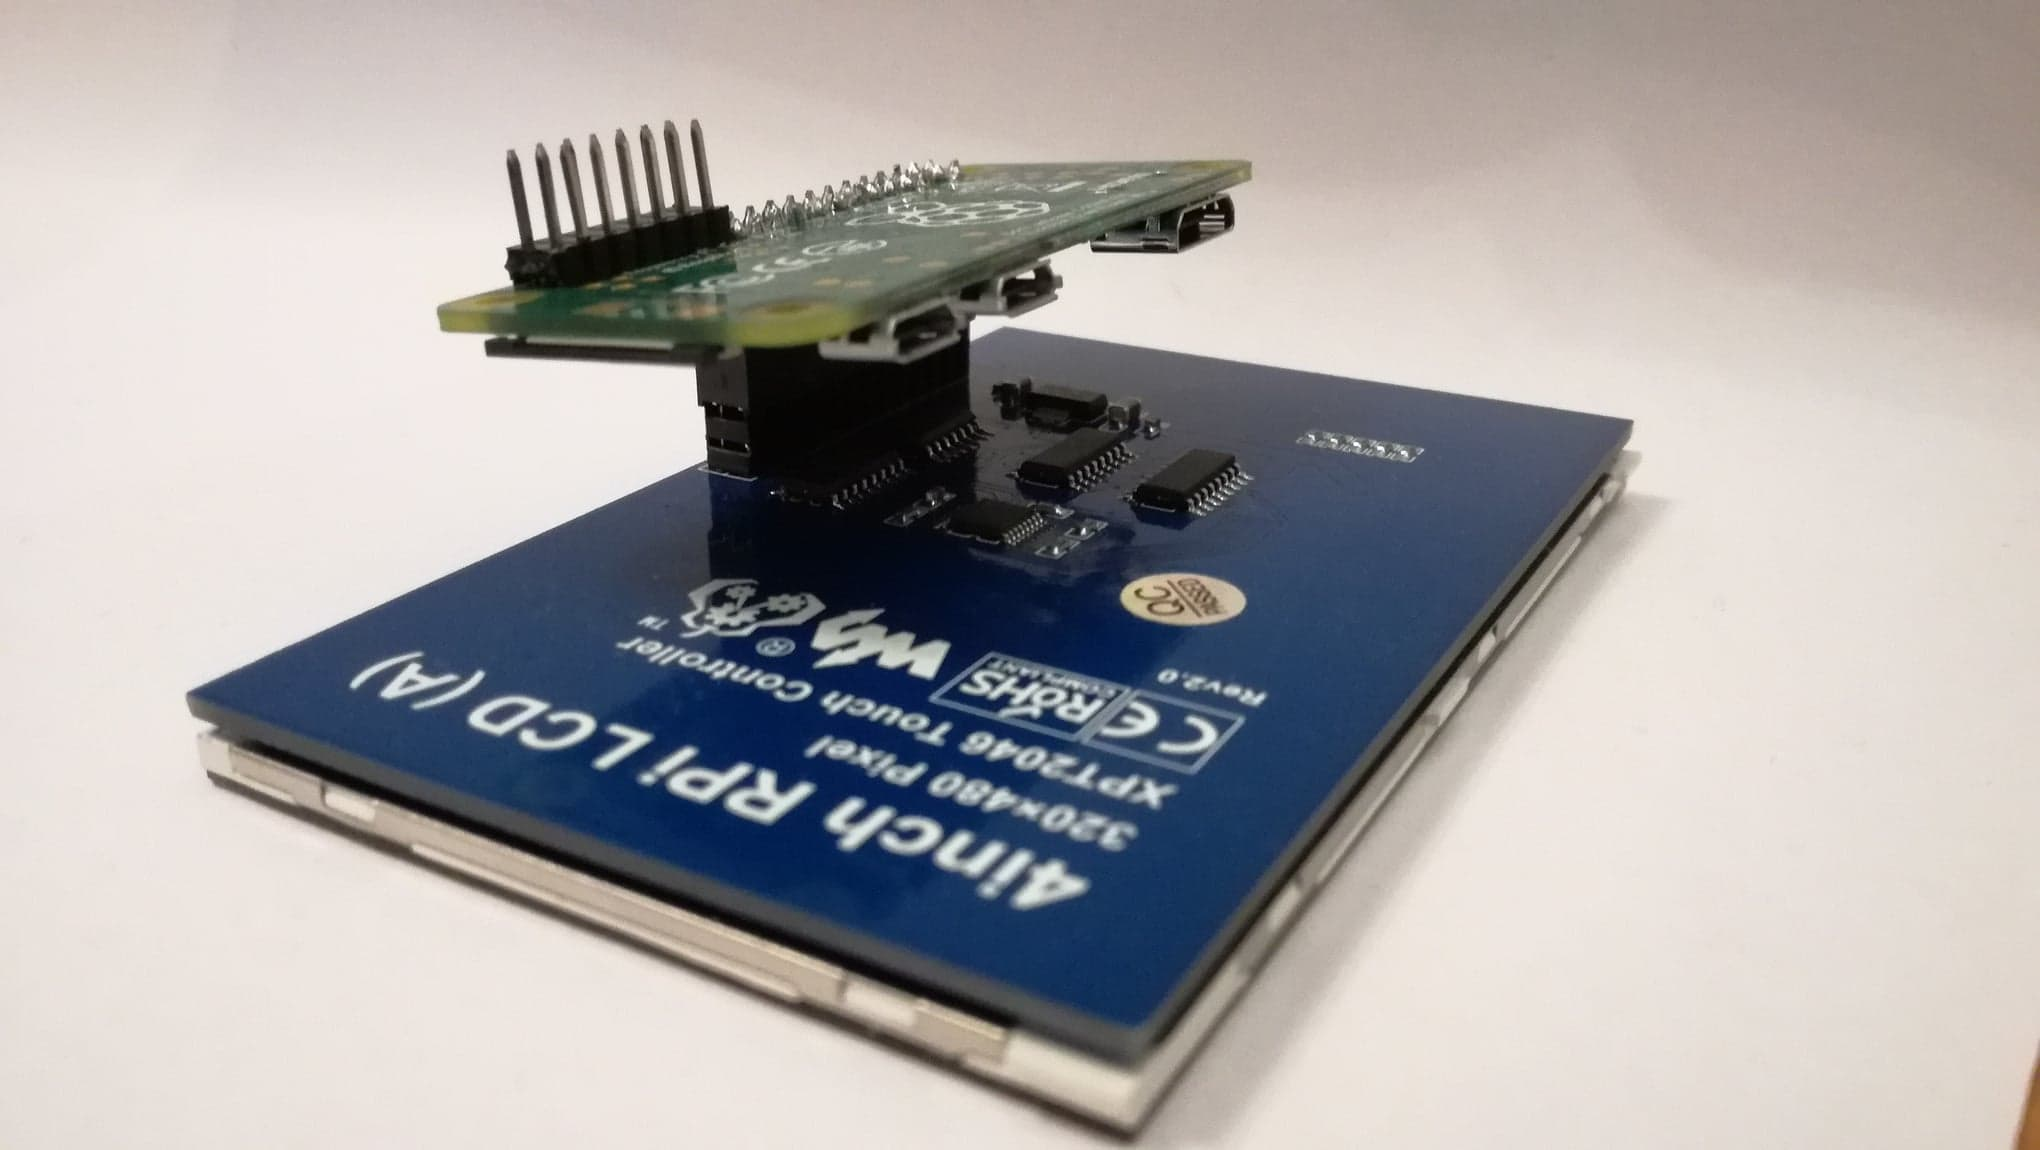
\includegraphics[scale=0.1]{rpi_lcd.jpg}
        		\caption{Połączenie Raspberry Pi z wyświetlaczem dotykowym} \label{fig:rpi_lcd} 
        	\end{minipage}
        \end{figure}
        \newpage \noindent
        \begin{figure}[H]
            \begin{center}
            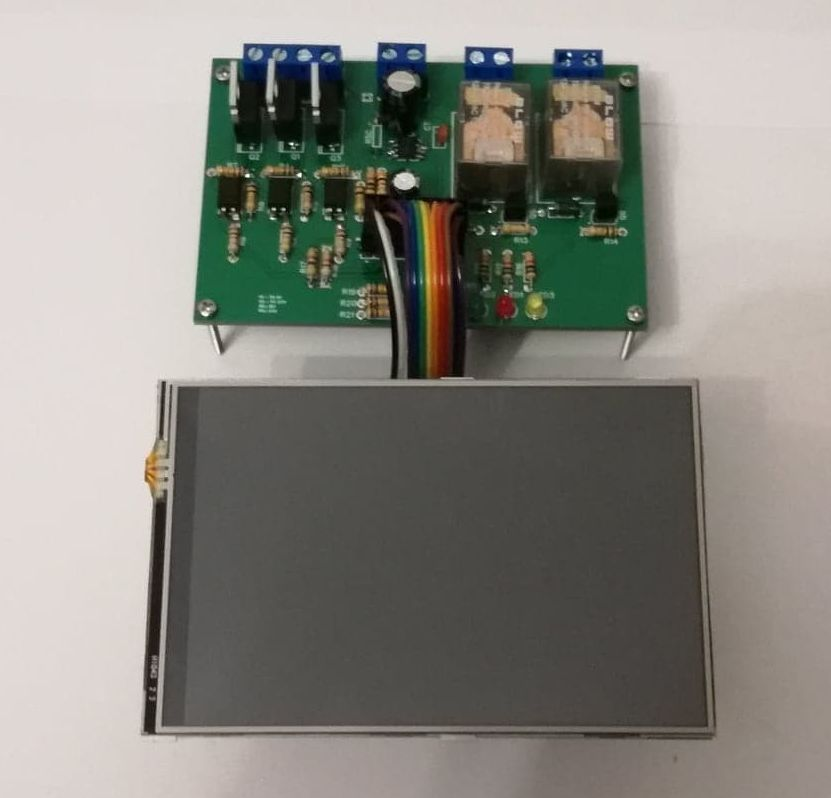
\includegraphics[width=0.6\textwidth]{poloczona_zoom.jpg}
            \caption{Moduł wykonawczy połączony z Rapsberry Pi}
            \end{center}
        \end{figure}
\noindent        Dzięki takiej budowie elementy wydzielające ciepło, takie jak tranzystory i procesor, mogą być od siebie oddalone. 

        
        \newpage
        \subsection{Tory wykonawcze}
            \subsubsection{Sterownik paska LED}
                Prototypownie modułu rozpoczęto od budowy sterownika paska ledowego, który sterowany był z prostego 8-bitowego mikrokontrolera \emph{Atmega 168P}. 
                Sterownik składa się z trzech identycznych kanałów, osobnego dla każdego koloru paska. 
                \begin{figure}[H]
                \begin{center}
                    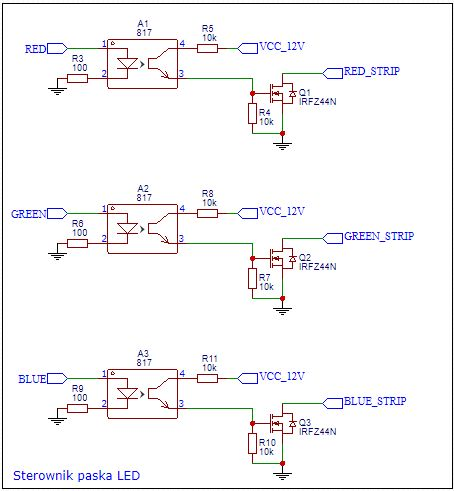
\includegraphics[width=0.8\textwidth]{sterownik1.jpg}
                    \caption{Schemat trzy kanałowego sterownika paska LED}
                \end{center}
                \end{figure}
                Elementem wykonawczym są tranzystory MOSFET (ang. Metal-Oxide Semiconductor Field-Effect Transistor), oznaczone na schemacie symbolami \emph{Q1}, \emph{Q2}, \emph{Q3}. Po podaniu między złącza bramka(ang. gate) i źródło(ang. source), określonego w nocie katalogowej\cite{irfz44nData} napięcia, tranzystor zaczyna przewodzić między złączami dren(ang. drain)-źródło. Należy pamiętać, że między drenem, a źródłem występuje rezystancja określona w nocie katalogowej symbolem Rds(on). Jest to ważny parametr, ponieważ ma on wpływ na ilość energii, która zostanie wytracona w formie ciepła, a co za tym idzie maksymalny prąd jaki tranzystor może przewodzić bez przegrzewania~się.
                \begin{figure}[H]
                \begin{center}
                    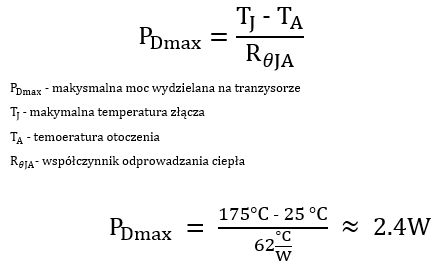
\includegraphics[width=0.6\textwidth]{obliczenia1.jpg}
                    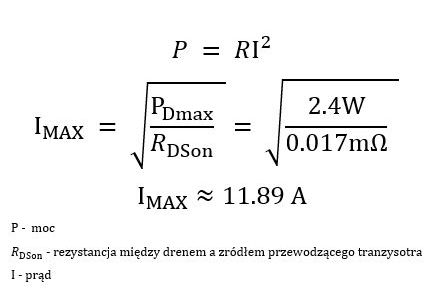
\includegraphics[width=0.6\textwidth]{obliczenia2.jpg}
                \end{center}
                \end{figure}
                \noindent Z powyższych obliczeń (na podstawie książki Sztuka elektroniki\cite{sztuka} ) wynika, że maksymalny prąd, który może przewodzić pojedynczy tranzystor (bez dodatkowego chłodzenia) to ponad 11A. Maksymalna moc sterownika paska led nie jest, więc uzależniona od wykorzystanych tranzystorów.  
                
            
            \subsubsection{Wyjścia przekaźnikowe}
            Moduł wyposażono również w dwa wyjścia przekaźnikowe pozwalające użytkownikowi na sterowanie stanem m.in. takich peryferiów jak: jednokolorowy pasek ledowy, żarówka led. W projekcie wykorzystano przekaźniki \emph{BLOW JQC-3F 12VDC}, dopuszają one przełączanie 10A prądu stałego przy 12V\cite{relData}.
            Moc cewki wybranych przekaźników wynosi 0.45W, więc w celu ich sterowania należało użyć tranzystor MOSFET. Niezbędnym elementem obwodu sterownika tranzystorowego przekaźników jest dioda, \emph{D3}, \emph{D4}, zabezpieczająca tranzystor przed energią znajdującą się w~cewce przekaźnika, który zostaje z niej wydalona pod wpływem zapadania się pola magnetycznego.
                \begin{figure}[H]
                \begin{center}
                    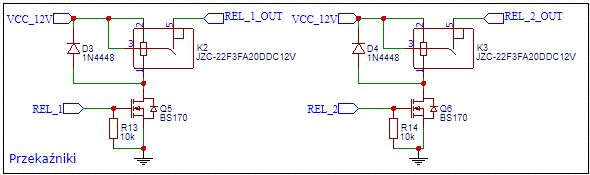
\includegraphics[width=0.9\textwidth]{przekazniki1.jpg}
                    \caption{Schemat wyjść przekaźnikowych}
                \end{center}
                \end{figure}
        \subsection{Przetwornica napięcia}
        Na płytce znajduje się także przetwornica napięcia, która służy zasileniu Raspberry Pi Zero. Zdecydowano się na wykorzystanie \emph{ON Semiconductor MC34063A} z~uwagi na dużą dostępność, niską cenę i łatwość użycia. Moduły MC34063 pracują w~zakresie napięcia wejściowego od 3V do 40V i~ mogą być skonfigurowane w~trybie obniżania, podwyższania lub odwracania napięcia. Maksymalny prąd wyjściowy to 1.5A, wartość ta przekracza potrzeby przy zasilaniu większości mikroprocesorów. Sterowanie parametrami układu DC-DC odbywa się przez dobór wartości elementów pasywnych. Nota katalogowa\cite{mc34063A} układu dostarcza potrzebne wzory potrzebne do obliczenia wartości elementów.
                \begin{figure}[H]
                \begin{center}
                    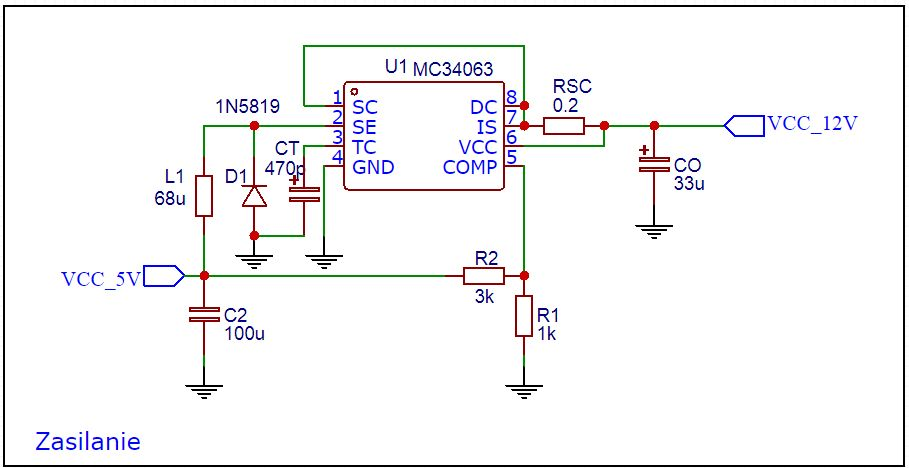
\includegraphics[width=0.75\textwidth]{zasilanie.jpg}
                    \caption{Schemat przetwornicy napięć}
                \end{center}
                \end{figure}
                
\noindent        Parametry wyjściowe układu przetwornicy z dobranymi elementami pasywnymi znajdują się tabeli \ref{tab:przet}.
             \begin{table}[H]
        \centering
        \begin{tabular}{ | m{15em} | m{3cm}| } 
        \hline
        Napięcie wejściowe & 12V \\ 
        \hline
        Napięcie wyjściowe & 5V \\ 
        \hline
        Częstotliwość  &55kHz\\
        \hline
        Wahania napięcia wyjściowego led &35mVpp\\
        \hline
        Maksymalny prąd wyjściowy &1500mA\\
        \hline
        \end{tabular}
        \caption{Parametry elektryczne modułu przetwornicy}
        \label{tab:przet}
        \end{table}
        
        \subsection{Elektronika dodatkowa}
        Na płytce umieszczono również elementy służące wyłącznie weryfikacji poprawności działania układu.
        
        \subsubsection{Przełącznik trybów pracy}
            \begin{figure}[H]
            \begin{center}
                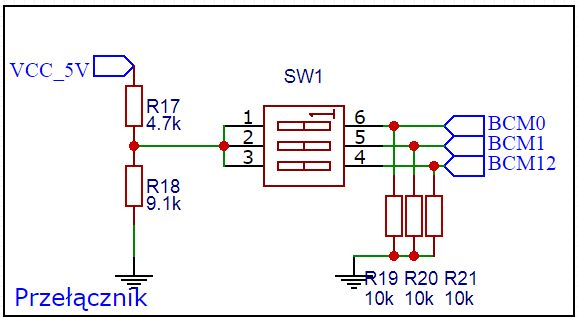
\includegraphics[width=0.6\textwidth]{przelacznik1.jpg}
                \caption{Schemat przełącznika trybów pracy}
            \end{center}
            \end{figure}
        W celu zmiany trybów diagnostycznych na płytce znajduje się potrójny przełącznik suwakowy. Z uwagi na 3.3V poziom logiczny Raspberry Pi i fakt, że na płytce znajduje się jedynie przetwornica napięcia o pięciowoltowym wyjściu należało stworzyć dzielnik napięciowy tworzony z rezystorów R17 i R18. Rezystory R19, R20, R21 są rezystorami podciągającymi.  
        \subsubsection{Diody sygnalizujące stan pracy}
            \begin{figure}[H]
            \begin{center}
                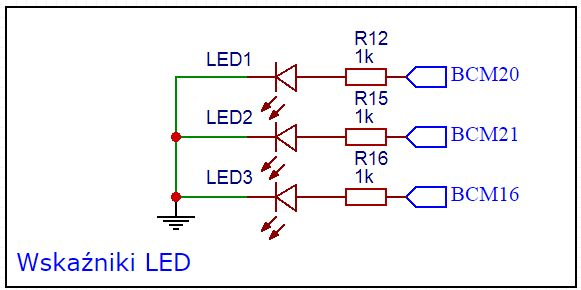
\includegraphics[width=0.6\textwidth]{wskaznik1.jpg}
                \caption{Schemat diod sygnalizacyjnych} 
            \end{center}
            \end{figure}
        Moduł posiada 3 diody sygnalizacyjne służące do informowania użytkownika o błędach lub mogące być wykorzystane przy sprawdzaniu modułu. Rezystory R12, R15, R16 dobrano tak aby intensywność świecenia diod nie oślepiała serwisanta badającego sterownik.\newpage
        
        \subsection{Wyświetlacz dotykowy}
        Zastosowanie wyświetlacza dotykowego w projekcie pozwala dodawać i zmieniać funkcjonalność produktu bez modyfikacji części fizycznej.
            \begin{figure}[H]
            \begin{center}
                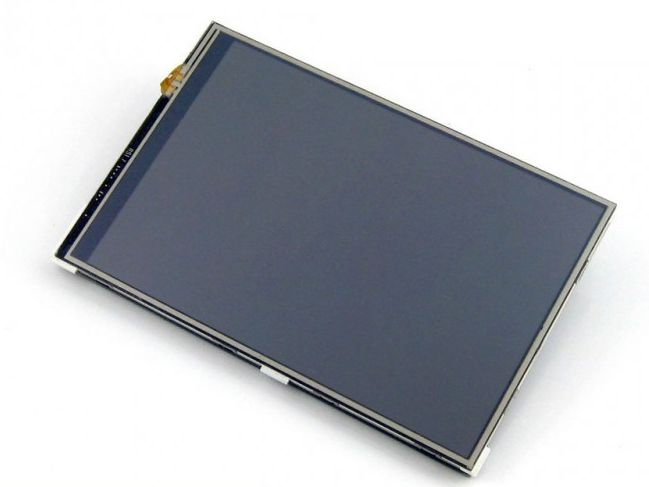
\includegraphics[width=0.6\textwidth]{wyswietlacz.jpg}
                \caption{Wyświetlacz dotykowy używany w module} 
            \end{center}
            \end{figure}
            
            \noindent W projekcie zdecydowano się na użycie gotowego modułu wyświetlacza dotykowego firmy
            \emph{Waveshare}. Jego rozmiar to 95 x 61 mm i posiada rozdzielczość 320x480 pikseli. Z~uwagi na te dwie własności, graficzny interfejs użytkownika został zaprojektowany tak aby wyświetlane informacje były czytelne. Komunikacja z Raspberry Pi odbywa się przez SPI. Produkt jest dedykowany do użytku z Raspberry Pi. Dokładniejsze przedstawienie sposobu działania jest niemożliwe, ponieważ produkt jest chroniony patentem i producent po za podstawową instrukcją obsługi\cite{screen} i sterownikami nie udostępnia dokumentacji technicznej.

        
        \subsection{Płytka drukowana}
            Po zakończonym etapie prototypownia poszczególnych partii, elementy te zostały połączone w jeden schemat, na podstawie którego zaprojektowano płytkę drukowaną (PCB). 
            Płytka ma wymiary 90x62mm, jest dwustronna, dzięki temu udało się zmniejszyć jej docelowy rozmiar. Na płytce znajdują się też złącza \emph{ARK} służące podłączaniu zasilania oraz urządzeń zewnętrznych. Maksymalny prąd, który może przewodzić złącze zasilania to 15A. Grubość poprowadzonych ścieżek zasilania do~modułu sterownika paska led pozwala na przewodzenie 12A prądu, natomiast do wyjść przekaźnikowych prąd ten (sumarycznie dla obu) wynosi 14A. 
    
    \newpage
        \subsection{Schemat połączeń z Raspberry Pi}
        Procesor \emph{BCM 2835} posiada 54 piny generalnego użytku\cite{RpiData}. Na płytce Raspberry Pi Zero W 1.3v wyprowadzone jest ich 26. Do obsługi peryferiów sterownika wykorzystano 11, komunikacja z wyświetlaczem zużywa ich 8, połączenia widoczne na rysunku \ref{fig:rpi_schm}.
            \begin{figure}[H]
            \begin{center}
                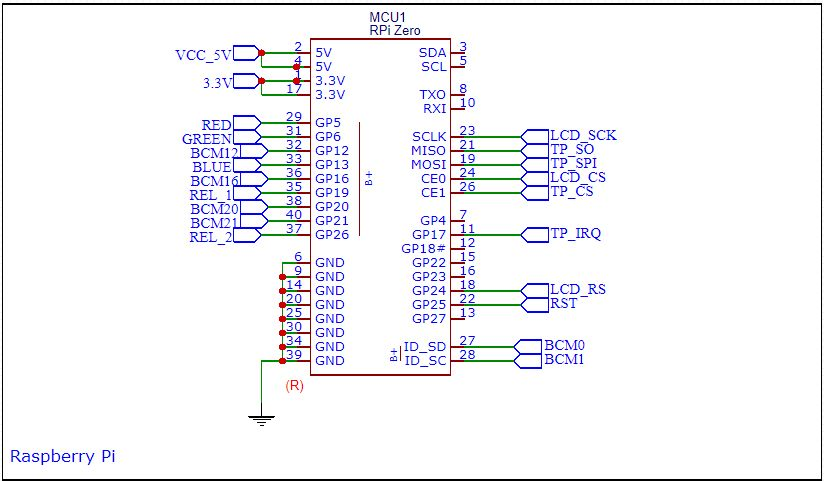
\includegraphics[width=0.8\textwidth]{rpi_schm.jpg}
                \caption{Schemat połączeń Rapberry Pi} \label{fig:rpi_schm} 
            \end{center}
            \end{figure}
        
    \section{Instrukcja montażu}
    Montaż układu powinno rozpocząć się od wizualnego sprawdzenia poprawności wykonania płytki drukowanej, ważnym jest sprawdzenie czy wszystkie punkty lutownicze są poprawnie pokryte i czy ścieżki nie wyglądają na uszkodzone, np. w transporcie.
    Pierwszym krokiem jest przylutowanie przetwornicy napięć, ponieważ jest to najmniejszy element i jej montaż może być później utrudniony przez sąsiadujące elementy. Dalej należy przylutować transoptory \emph{A1}, \emph{A2}, \emph{A3}.  Następnie w dowolnej kolejności można przylutować: rezystory \emph{R1} do \emph{R21}, kondensatory \emph{C0}, \emph{Ct}, \emph{C2}, diody \emph{D1}, \emph{D3}, \emph{D4}, tranzystory \emph{Q1}, \emph{Q2}, \emph{Q3}, \emph{Q5}, \emph{Q6}, diody led \emph{LED1}, \emph{LED2}, \emph{LED3}. Po wykonaniu tych czynności należy przylutować złącze \emph{JP1}, przełącznik suwakowy \emph{SW1}, złącza ARK \emph{J1} - \emph{J5}. Ostatnimi elementami na górnej warstwie są przekaźniki \emph{K2}, \emph{K3}. Na dolej warstwie płytki powinna znaleźć się cewka \emph{L1} i rezystor \emph{RSC}, tak~jak jest to widoczne na \ref{fig:pcb_dol}. 
    Złącza goldpin na Raspberry Pi powinne zostać polutowane tak aby piny od 27 do 40 były skierowane w kierunku przeciwnym do mikroprocesora na płytce (patrz \ref{fig:rpi1}), pozostałe odwrotnie. 
            \begin{figure}[H]
            \begin{center}
                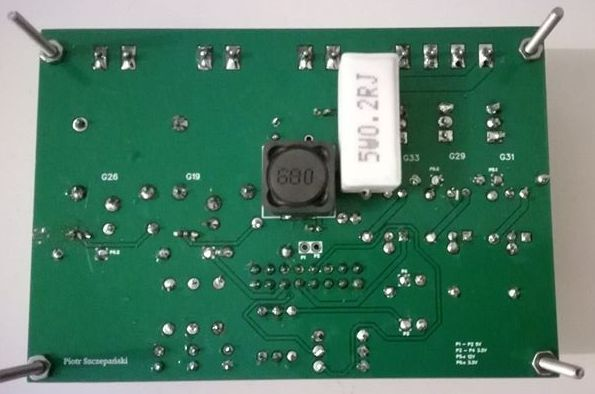
\includegraphics[width=0.5\textwidth]{dol.jpg}
                \caption{Dolna warstwa płytki} \label{fig:pcb_dol} 
            \end{center}
            \end{figure}
\noindent    Montaż wyświetlacza dotykowego do płytki Raspberry Pi odbywa się przez wsunięcie go w złącze goldpin, poprawna instalacja widoczna jest na \ref{fig:rpi_lcd}. Komunikacja płytki sterującej z płytką wykonawczą odbywa się przez 16-sto żyłowy kabel, który od strony płytki wykonawczej powinien być zakończony damski złączem 2x8 goldpin, a na drugim końcu złączem 2x7 oraz dwoma przewodami, które muszą zostać przylutowane do pinów 3 (5V) i 4 (GND) na Raspberry Pi. 
\newpage

    \section{Sprawdzanie modułu}
            Płytka i opis znajdujący się na niej został zaprojektowany tak, aby w łatwy sposób można było sprawdzić poprawność działania modułu. 
            
            \subsection{Sprawdzanie poprawności działania modułu wykonawczego}
            Dolna strona PCB zawiera dwa rodzaje oznaczeń, które służą do sprawdzenie poprawności działania elektroniki płytki:
            \begin{itemize}
                \item oznaczenia \emph{G*} informujące do którego pinu mikroprosesora podłączone jest dany element modułu, ma to ułatwić programowanie i sprawdzanie poprawności konfiguracji peryferiów,
                \item oznaczenia \emph{P*} będące punktami testowymi.
            \end{itemize}
               \begin{figure}[H]
                \begin{center}
                    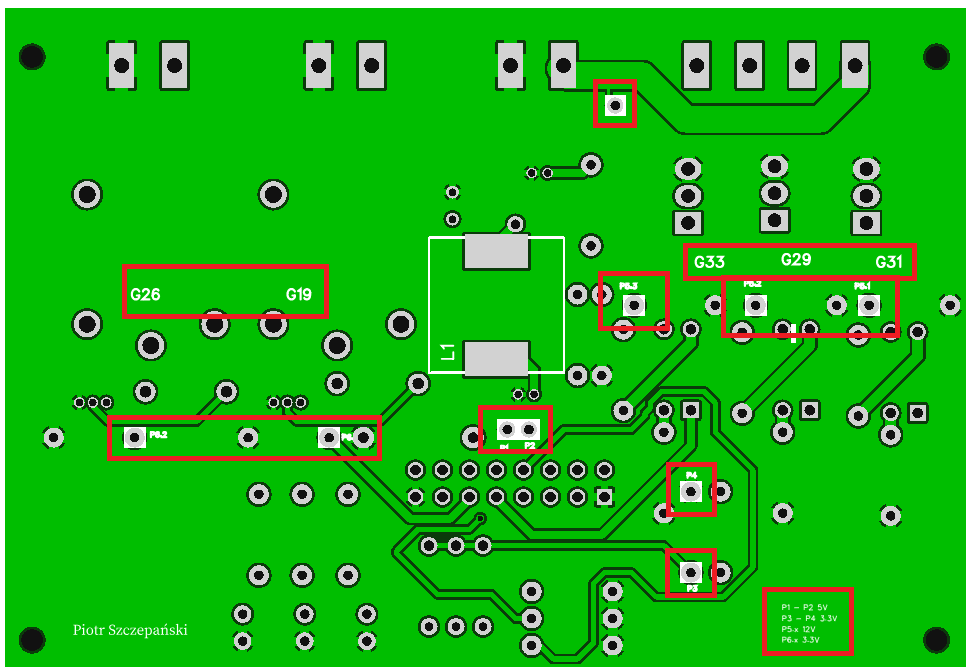
\includegraphics[width=0.6\textwidth]{pcb_dol_zaz.png}
                    \caption{Punkty kontroli poprawności działania}
                \end{center}
                \end{figure}
            Na płytce znajduje się, również oznaczenie mówiące o poprawnych wartościach między punktami kontrolnymi \emph{P1} - \emph{P4} oraz napięcia, które należy podać między masą a punktami \emph{P5} - \emph{P6}.
            Sprawdzenie poprawności montażu elementów przetwornicy napięcia, odbywa się przez pomiar napięcia między punktami P1 P2, napięcie to powinno wynosić 5V z  pięcioprocentową dokładnością.
            Należy również sprawdzić wartość napięcia między punktami P3 P4, które powinno wynosić 3.3V.
            W celu sprawdzenia sterownika paska LED należy podać 12V kolejno między masą, punktami P5.1, P5.2, P5.3~i~mierzyć napięcie na odpowiadających wyjściach sterownika. Moduł działa poprawnie jeśli napięcie na wyjściu każdego z kanałów będzie równe 12V.
            Sprawdzenie wyjść przekaźnikowych odbywa się przez podanie 3.3V, z punktu P4, na punkty P6.1 i P6.2.
            Przekaźnik w momencie przełączania wydaje wyraźny dźwięk (kliknięcie), więc jego brak w chwili podłączenia napięcia oznacza niepoprawne działanie. Kolejnym etapem weryfikacji jest zmierzenie napięcia na wyjściach przekaźnikowych przy zwartych P6.1 lub P6.2 z P4, powinno ono być równe 12V. Opisane metody testowania nie wymagają podłączenie Raspberry Pi, ale wymagają podłączenie zasilania 12V. 
            
            \subsection{Sprawdzenie poprawności działania całości modułu}
                \begin{figure}[H]
                \begin{center}
                    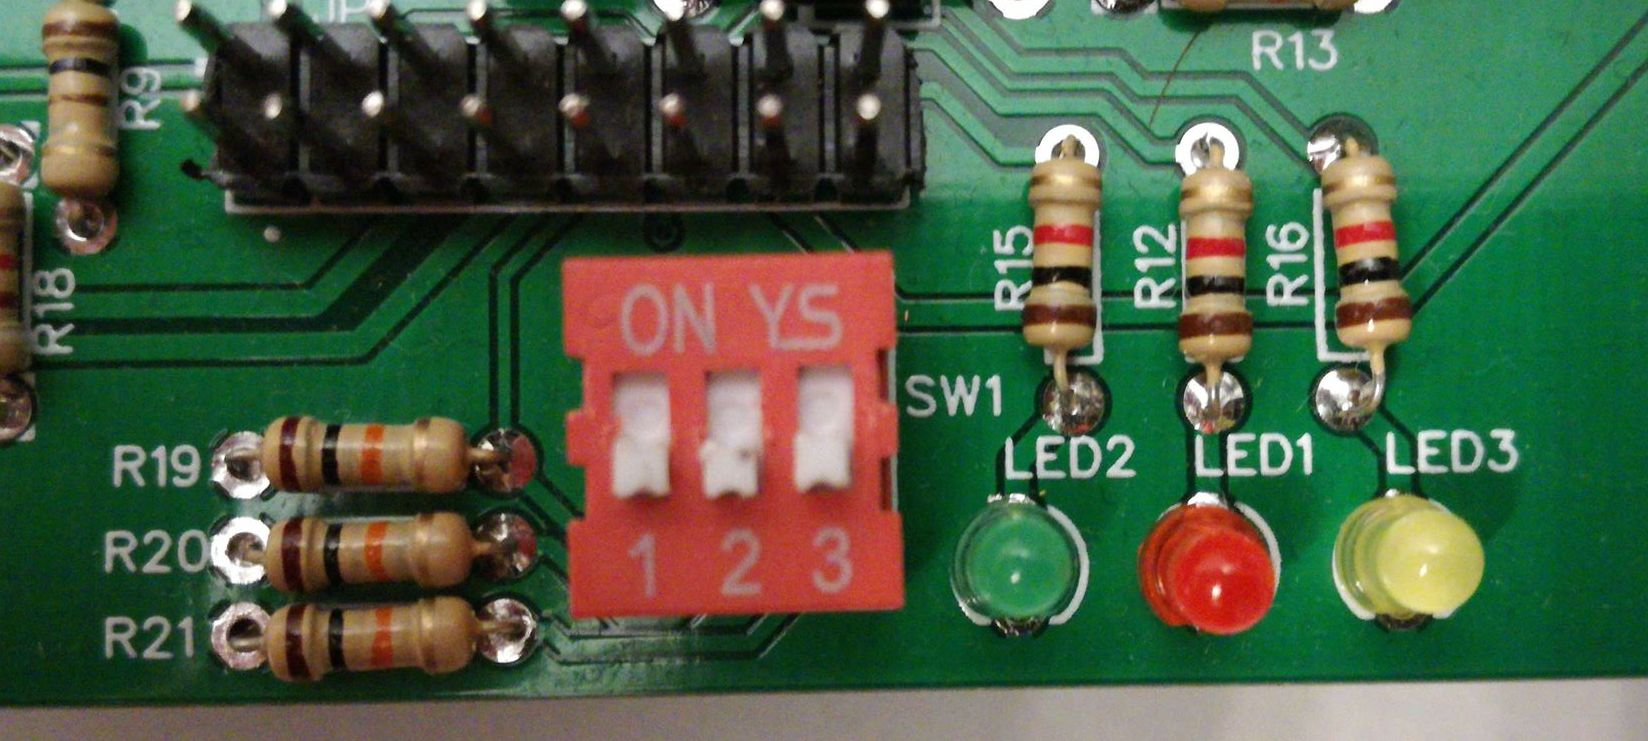
\includegraphics[width=0.5\textwidth]{dip_zoom.jpg}
                    \caption{Przełącznik trybów i diody sygnalizacyjne}
                \end{center}
                \end{figure}
            Sterownik udostępnia 3 tryby serwisowe wybierane za pomocą przełącznika suwakowego.
            Oprogramowanie sterownika odczytuje wartości wejść, do których podłączony jest przełącznik, w momencie startu systemu, więc aby włączyć tryb serwisowy należy odłączyć zasilanie modułu, wybrać tryb i podłączyć zasilanie. Nie jest dozwolone przełączenie dwóch lub więcej przełączników. W takim przypadku system zignoruje te informacje i uruchomi moduł w trybie pracy normalnej. Przejście modułu w tryb serwisowy sygnalizowane jest ciągłym podświetleniem diody \emph{LED3}.
            
            Dostępne tryby:
            \begin{itemize}
                \item przełącznik w pozycji 1 - w trybie tym sterownik będzie włączał i wyłączał z odstępem 1 sekundy wyjścia modułu w kolejności : kanał czerwony, kanał zielony, kanał niebieski, wyjście przekaźnikowe 1, wyjście przekaźnikowe 2. Tryb ten pozwala sprawdzić poprawność działania elektroniki wyjściowej oraz podłączenia modułu Raspberry Pi.
                
                \item przełącznik w pozycji 2 - tryb jest przeznaczony do sprawdzenia poprawności działania wyświetlacza, w~ szczególności poprawności wyświetlania kolorów, czasu odświeżania, dokładności powierzchni dotykowej.
                Na ekranie wyświetli się licznik inkrementujący swoją wartość od 0 do 10000 co 200ms, napis "TEST"~w 3 rozmiarach oraz tło aplikacji będzie zmieniało kolory z częstotliwością 500ms w~ kolejności: czerwony, zielony, niebieski, biały. Ponadto na ekranie widoczne będą 4 pola dotykowe, których naciśnięcie będzie aktywowało diodę \emph{LED2},~w~przypadku wykrycia dotyku po za, którymś z tych pól załączona zostanie dioda \emph{LED1}. 
                
                \item przełącznik w pozycji 3 - tryb służący do kontroli obciążenia procesora systemu, zajętości RAM-u oraz temperatury na procesorze. Informacje te będą wyświetlane na ekranie. Dodatkowo zostanie wyświetlony plik kontrolny z~poprzedniego uruchomienia modułu.
            \end{itemize}
            
\noindent            Wyłączenie trybu serwisowego jest możliwe dopiero po odłączeniu zasilania i~ustawieniu przełącznika serwisowego do konfiguracji pracy standardowej.
            Moduł ignoruje zmiany przełącznika suwakowego w czasie działania programów.
            
            \newpage
            
            \section{Dokumentacja oprogramowania}
            Kompletny zestaw wytworzonego oprogramowania modułu składa się z pięciu plików binarnych - jednego dla programu użytkownika, trzech dla każdego z trybów serwisowych, jednego służącego do konfiguracji peryferiów oraz ze skryptu bash'owego wykorzystywanego przy starcie modułu.
            
                \subsection{Interfejs graficzny}
                Interfejs graficzny jest w całości napisany w języku QML korzystając z biblioteki QtQuick w~ wersji~ 2.6\cite{qtQuick2.6}, za paletę kolorów interfejsu odpowiada biblioteka Material~2.0\cite{qtMaterial2}, kształt i zachowania elementów widoku zaczerpnięto z biblioteki Controls~2.0 \cite{qtControls2}. 
                
                \subsubsection{Przykład połączenia klasy C++ z QML}
                Przykład demonstruje mechanizm łączenia klas C++ z~kodem interfejsu graficznego w QML, z~uwagi na zbyt dużą złożoność kodu w projekcie, posłużono się uproszczoną wersją. Kod przykładu pokazuje obsługę przełącznika (Switch) takiego jak wykorzystany na Rys \ref{fig:view5}.
                    \begin{figure}[H]
                    \begin{center}
                        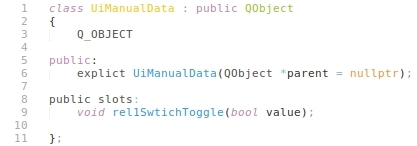
\includegraphics[width=0.65\textwidth]{code_class.jpg}
                    \end{center}
                    \end{figure}
\noindent                    Klasa UiManualData ma reagować na zmianę stanu przełącznika w sposób asynchroniczny, aby to osiągnąć należy skorzystać z modelu sygnałów i slotów z QT. Tworząc własny typ uzyskuje się to poprzez dziedzicznie po typie QObject oraz definicję makra Q\_OBJECT w sekcji prywatnej klasy. W lini 9 znajduje się definicja slotu, który będzie wywoływany z obiektu QML.
                    
                    \begin{figure}[H]
                    \begin{center}
                        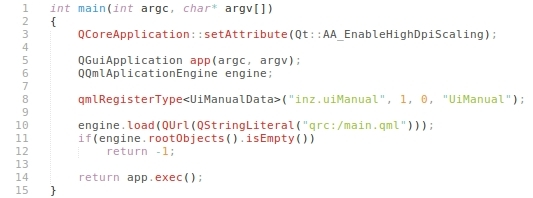
\includegraphics[width=0.65\textwidth]{code_main.jpg}
                    \end{center}
                    \end{figure}
\noindent                    W celu udostępnienia klasy UiManualData w QML, należy ją zarejestrować, czynność ta odbywa się w linijce 8.
                    
                    \begin{figure}[H]
                    \begin{center}
                        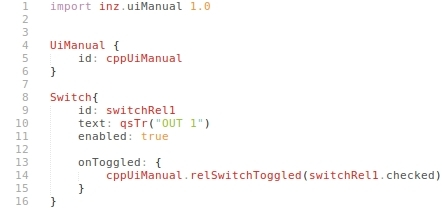
\includegraphics[width=0.65\textwidth]{code_qml.jpg}
                    \end{center}
                    \end{figure}
      \noindent              W pliku .qml trzeba zaimportować klasę, linia 1, pamiętająć o numerze wersji z~ jakim zarejestrowało się dany typ. Następnie trzeba stworzyć obiekt tej klasy, linijki 4-6.
                    Po wykonaniu tych czynności można korzystać z interfejsu klasy. W~sygnale \emph{onToggle} (sygnał wywoływany przy zmianie stanu przełącznika) obiektu Switch, występuje wywołanie metody klasy UiManualData.
                
                \newpage
                
                
                \subsection{Struktura oprogramowania użytkowego}
                Zaplecze oprogramowania zaprojektowano w formie warstw funkcjonalności, widoczne na rysunku \ref{fig:layers}. Podział ten widać na Rys \ref{fig:layers}. Dokumentowanie oprogramowania w taki sposób definiuje jedynie logiczny podział kodu oraz przepływ informacji i nie dezaktualizuje się przy dodawaniu nowych funkcjonalności\cite{CleanCode}.  
                    \begin{figure}[H]
                    \begin{center}
                        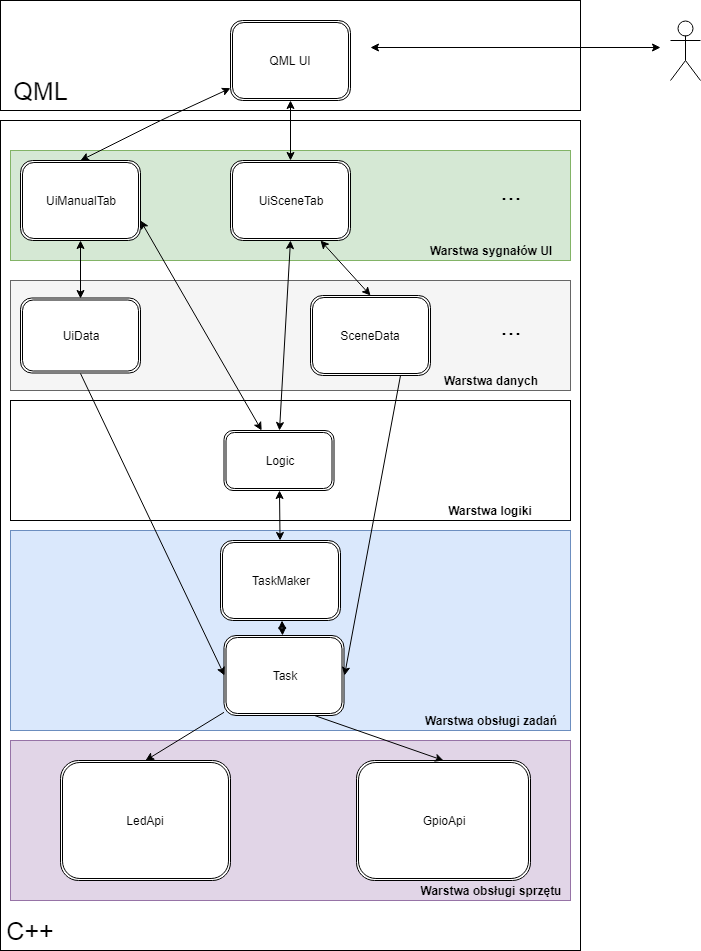
\includegraphics[width=0.7\textwidth]{inz_diag1.png}
                        \caption{Schemat warstwowy oprogramowania trybu normalnego~użytku} \label{fig:layers}
                    \end{center}
                    \end{figure}
                \subsubsection{Warstwa sygnałów UI}
                Warstwa sygnałów UI jest bezpośrednim połączeniem z interfejsem graficznym QML. Wykorzystywane są tutaj takie mechanizmy jak ten przedstawiony w sekcji 5.5.1. Warstwa ta jest całkowicie przezroczysta - nie przechowywane są tutaj żądane dane oraz nie ma w niej zaimplementowanej logiki systemu. Sprawdzane jest jedynie czy dane przychodzące z warstwy UI są poprawne.
                
                \subsubsection{Warstwa danych}
                Warstwa danych przechowuje dane wprowadzone przez użytkownika takie jak: konfiguracja scen i~ alarmów, obecny stan modułu oraz dane animacji.  
                
                \subsubsection{Warstwa logiki}
                Warstwa logiki jest prostą maszyną stanów, która podejmuje decyzje na podstawie sygnału z~ interfejsu użytkownika jak i z informacji o obecnym stanie urządzenia. Na przykład jeśli użytkownik ręcznie uruchomi animację i w~trakcie jej wykonywania zostanie aktywowany alarm, zostanie zlecone przerwanie wykonywania animacji i~wywołana będzie zadana funkcja alarmu.
                
                \subsubsection{Warstwa obsługi zadań}
                Warstwa obsługi zadań odpowiada za planowanie i~wykonywanie czynności zadanych przez warstwę logiki. Dane do poszczególnych zadań pobierane są bezpośrednio z~warstwy danych.
                
                \subsubsection{Warstwa obsługi sprzętu}
                Warstwa obsługi sprzętu jest jednie abstrakcją do sprzętu urządzenia, wykonuje zlecone polecenia. Nie podejmuje, żadnych decyzji, mogąc jedynie zgłosić błąd wykonywania czynności.
                
                    \newpage
                \subsection{Obsługa sprzętu}
                Do obsługi sprzętu zdecydowano się użyć bibliotekę WiringPi \cite{wiringPi}, która jest udostępniana na zasadach \emph{GNU LGPL v.3 }. Biblioteka jest napisana proceduralnie w~języku C i~stanowi jedynie warstwę abstrakcji do sprzętu mikroprocesora. W spiera używanie mikroprocesorów \emph{BCM2835}, \emph{BCM2836} oraz  \emph{BCM2837}. \\*
                WiringPi implementuje m.in. : 
                \begin{itemize}
                    \item obsługę wejść i wyjść,
                    \item obsługę przerwań,
                    \item PWM,
                    \item SPI,
                    \item IIC,
                    \item wielowątkowość.
                \end{itemize}
                W projekcie wykorzystano jedynie obsługę PWM.
                
                \subsection{Oprogramowanie dodatkowe}
                W celu kontroli działania modułu stworzono dodatkowe oprogramowanie służące jednie inwestygacji niesprawności w module.
                \subsubsection{Logger}
                Klasa \emph{Logger} pozwala na zapisywanie, w pliku tekstowym w ustalonym formacie, informacji o zdarzeniach w oprogramowaniu.  Interfejs klasy udostępnia decydowanie o poziomie krytyczności wiadomości.
                    \begin{figure}[H]
                    \begin{center}
                        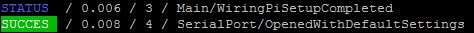
\includegraphics[width=0.9\textwidth]{logger.jpg}
                        \caption{Przykładowy wycinek pliku loggera}
                    \end{center}
                    \end{figure}
                \noindent Kolejne pola oznaczają status wiadomości, czas od startu programu w sekundach, liczba porządkowa wiadomości oraz treść wiadomości.
                
                \subsubsection{Pomiar obciążenia systemu}
                W celu diagnostyki systemu Linux stworzono klasę badającą obciążenie zasobów systemowych. Klasa pozwala na badanie obciążenia procesora, procentu zajętości pamięci RAM i monitorowanie temperatury na procesorze.
                
                \newpage
                
                \subsection{Opis scenariuszy programowych}
                W oprogramowaniu modułu znajduje się cztery scenariusze programowe, których kolejność i~sposób wykonywania jest kluczowy w procesie sprawdzania poprawności działania modułu i~kontroli jakości. Opisany nie został program użytkowy modułu z~uwagi na zależność od zachowań użytkownika oraz asynchroniczność jego działania.
                    \subsubsection{Start modułu}
                    Start modułu jest krytycznym momentem, który decyduje o całości działania modułu.
                        \begin{figure}[H]
                        \begin{center}
                            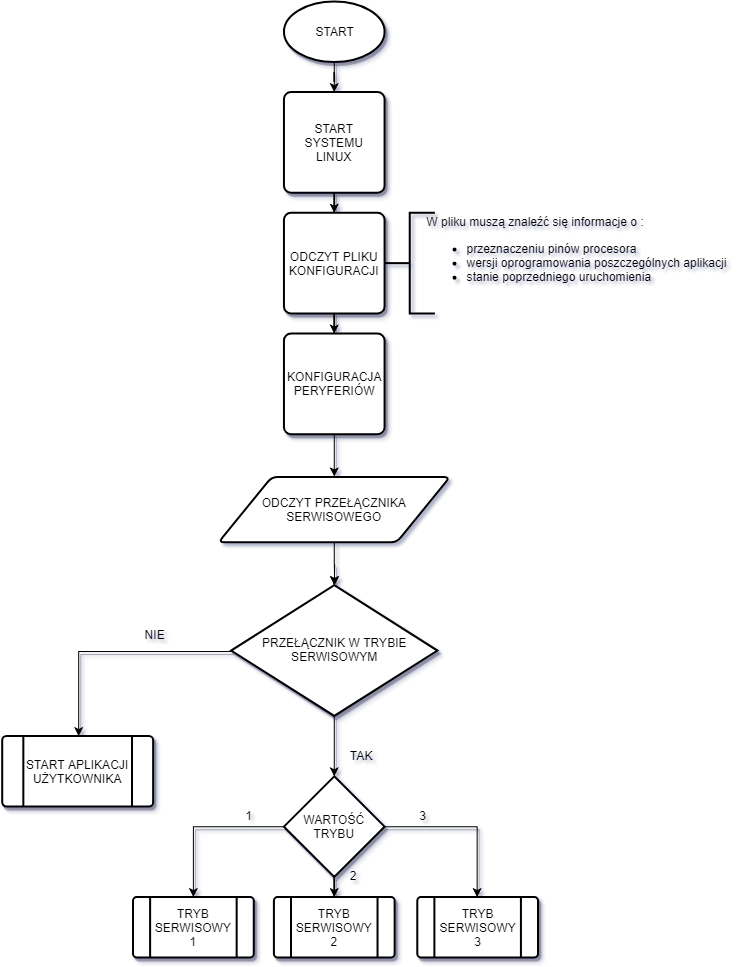
\includegraphics[width=0.7\textwidth]{startup.png}
                            \caption{Schemat blokowy startu modułu} \label{fig:startup}
                        \end{center}
                        \end{figure}
                Przedstawiony schemat blokowy (rysunek \ref{fig:startup}) jest zaimplementowany w postaci skryptu bash'owego uruchamianego bezpośrednio po starcie systemu operacyjnego. Decyduje on o~trybie uruchomienia urządzenia, włącza odpowiedni plik binarny i~konfiguruje peryferia sprzętowe procesora.
                \newpage
                        
                    \subsubsection{Tryb serwisowy 1}
                    Osobny program służący do testowania połączenia Raspberry Pi z~modułem wykonawczym, nie wykorzystuje kodu źródłowego aplikacji użytkownika.Napisano go w~taki sposób aby zminimalizować możliwość wystąpienia błędu w czasie działania.
                        \begin{figure}[H]
                        \begin{center}
                            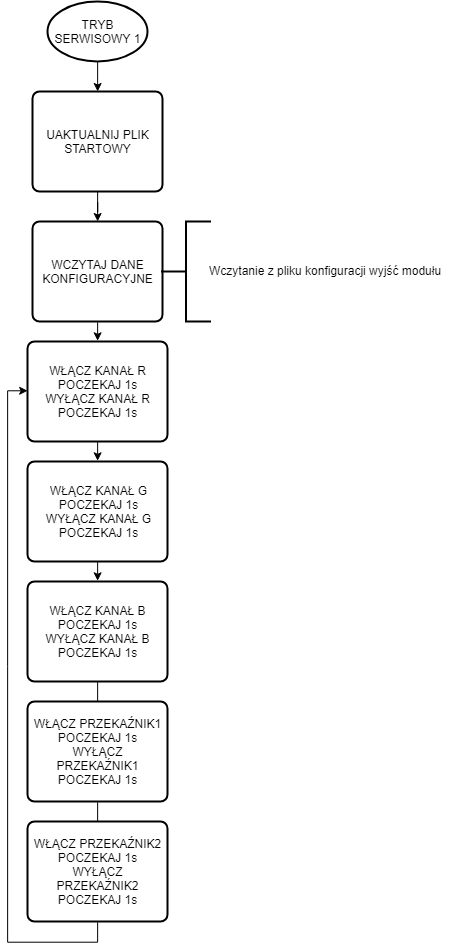
\includegraphics[width=0.4\textwidth]{t1.png}
                            \caption{Schemat blokowy trybu serwisowego 1} \label{fig:serT1}
                        \end{center}
                        \end{figure}
                        \noindent Program umieszcza w pliku kontrolnym informację, że sterownik został uruchomiony w trybie testowym. Opis testu znajduje się w sekcji 5.3.2. 

                        \newpage
                    
                    \subsubsection{Tryb serwisowy 2}
                    Program służy do całościowego testowania modułu (dokładniejszy opis testu w~sekcji 5.3.2). Jest on osobnym programem, który korzysta z logiki i~implementacji wykorzystanych w~aplikacji użytkownika.
                        \begin{figure}[H]
                        \begin{center}
                            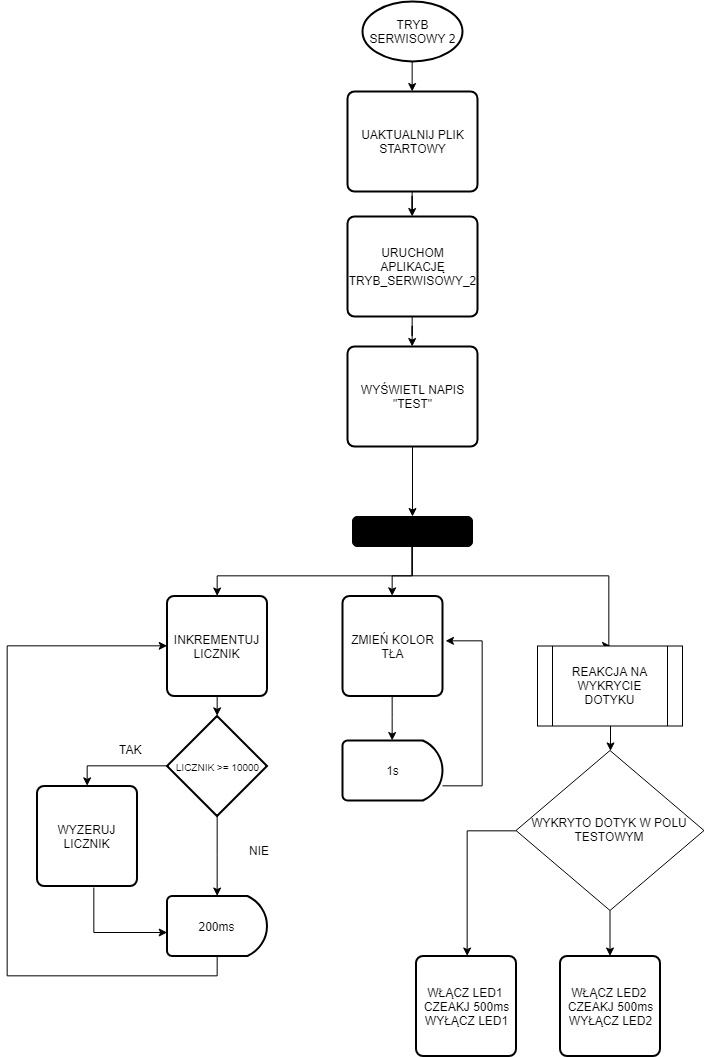
\includegraphics[width=0.7\textwidth]{t2.png}
                            \caption{Schemat blokowy trybu serwisowego 2} \label{fig:serT2}
                        \end{center}
                        \end{figure}
                    Program składa się z trzech zadań wykonywanych równolegle. Testu sprawności i kalibracji wyświetlacza dotykowego. Zmiany koloru tła, pozwalającego sprawdzić poprawność wyświetlanych kolorów oraz szybkości odświeżania wyświetlacza.
                        \newpage
                        
                    \subsubsection{Tryb serwisowy 3}
                    Opis scenariusza testowego znajduje się w sekcji 5.3.2.
                        \begin{figure}[H]
                        \begin{center}
                            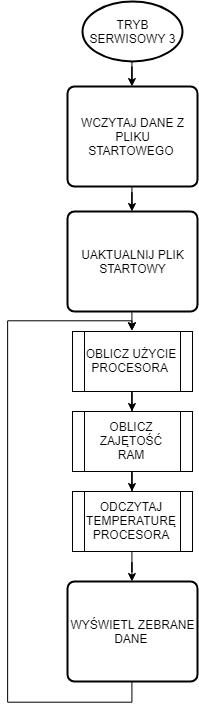
\includegraphics[width=0.25\textwidth]{t3.png}
                            \caption{Schemat blokowy trybu serwisowego 3} \label{fig:serT3}
                        \end{center}
                        \end{figure}
                        \noindent Program ten swoje działanie rozpoczyna od odczytanie pliku startowego z~poprzedniego uruchomienia aplikacji użytkownika, wyświetla on następnie takie dane jak czas poprzedniego działania, błędy, oprócz tego program wyświetla na ekranie dotykowym, dane o~chwilowym obciążeniu systemu.
                    
                        \newpage

\chapter{Wnioski i uwagi}
Zgodnie założeniami projektowymi powstało urządzenie, które realizuje postawione wymagania oraz spełnia zadane kryteria jakościowe. W ramach prac nad urządzeniem powstała również dokumentacja techniczna i opis wykorzystanych technologi. Proces prototypownia, projektowania i tworzenia modułu wraz z jego dokumentacji dostarczył cennych obserwacji i wniosków. W szczególności zaobserwowano, że:
\begin{itemize}

\item Wszystkie wykorzystane w projekcie technologie są standardem w branży produkcji urządzeń wbudowanych. Zastosowanie języka C++ pozwoliło stworzyć oprogramowanie, które będzie łatwo rozszerzalne w przyszłości o nową funkcjonalność. Biblioteka QT i język QML dały możliwość zrealizowania czytelnego i responsywnego interfejsu graficznego. Wykorzystanie Raspberry Pi Zero W ułatwiło proces tworzenia oprogramowania, natomiast platforma ta nie byłaby odpowiednia do produktu konsumenckiego z uwagi na zbyt duży koszt w masowej produkcji. Raspberry Pi Zero W nie pozwoliłoby również na rozszerzenie części sprzętowej urządzenia. Rozwiązaniem tego problemu byłoby dołożenie mikroprocesora sterującego tylko elektroniką, który komunikowałby się z modułem nadrzędnym.

\item Projekt posiada większą funkcjonalność niż standardowe urządzenia tego typu, agregują sterownik paska ledowego oraz dwa programowalne moduły przekaźnikowe. Zdolność elektryczna modułu jest kilkukrotnie wyższa niż podobnych urządzeń na rynku i pozwalałoby sterować oświetleniem małego pomieszczenia użytkowego.

\item Interfejs graficzny użytkownika pomimo zastosowania stosunkowo małego wyświetlacza pozostaje czytelny, korzystanie z niego jest intuicyjne. Dostępne funkcje i ich obsługą oferują użytkownikowi różnorodność w sposobach wykorzystania modułu. 

\item Zaprojektowana elektronika poprawnie spełnia założoną funkcjonalność. Tranzystory MOSFET pozwalałyby przełączać większe obciążenie, natomiast ograniczeniem jest płytka drukowana i zastosowane złącza. Wyświetlacz dotykowy w przyszłości mógłby być zastąpiony większym lub całkowicie zlikwidowany na rzecz aplikacji w urządzeniu mobilnym. Dodatkowo elektronika modułu mogła by oferować pomiar zużywanej energii oraz czujniki ruchu.

\item Sposób zaprojektowania elektroniki pozwala na łatwiejsze sprawdzanie poprawności działania. Instrukcja montażu w dokładny sposób tłumaczy kolejne kroki budowy modułu. W przyszłości wszystkie elementy przewlekane mogłyby zostać zastąpione montowanymi powierzchniowo w celu automatyzacji procesu konstrukcji produktu.

\item Stworzone oprogramowanie jest zgodne z panującymi zasadami tworzenia kodu. Podział warstwowy umożliwia łatwe rozszerzanie o dodatkową funkcjonalność. Zastosowanie języka QML pozwoliło utworzyć , Zastosowanie biblioteki WiringPi dało możliwość szybkiego oprogramowania warstwy obsługi sprzętu, niestety biblioteka ta nie jest przenośna między platformami i sposób jej implementacji nie pozwala na korzystanie z bardziej zaawansowanych aspektów peryferiów mikroprocesora.

\end{itemize}
\thispagestyle{fancy}



\listoffigures
\listoftables
\bibliographystyle{plabbrv}

\addcontentsline{toc}{chapter}{Bibliografia} %utworzenie w spisie treści pozycji Bibliografia
\bibliography{bibliografia} % wstawia bibliografię korzystając z pliku bibliografia.bib - dotyczy BibTeXa, jeżeli nie korzystamy z BibTeXa należy użyć otoczenia thebibliography



\end{document}